\documentclass[12pt,letterpaper]{article}

\usepackage{amsmath, amsthm, amsfonts, amssymb}
\usepackage{microtype, parskip, graphicx}
\usepackage[comma,numbers,sort&compress]{natbib}
\usepackage{lineno}
\usepackage{longtable}
\usepackage{docmute}
\usepackage{caption, subcaption, multirow, morefloats, rotating}
\usepackage{wrapfig}
\usepackage{hyperref}

\frenchspacing

\begin{document}

\section{Results}

\subsection{Posterior predictive results}
% why do i want to show all these graphs?
%   demonstrate how well the model recapitulates the observed data
%   if the model simulates datasets like the one we observed
%     then we can be more confident in our inferences
%   PPCs by group reveal even more about the fit of our model
%     are some time bins better predicted by others?
%     well predicted time bins indicate congruence with model assumptions
%     poorly predicted time bins indicate incongruence with model assumptions
%       something different is happening in these bins that requires explanation



Overall, the expected taxonomic diversity of geological units for each taxonomic group is adequately described by the fitted models, where adequacy means that the posterior predictive distribution of our models resemble the empirical data. While there are aspects of misfit when considering their entire distribution, the aspects of the distribution which are critical to our analysis are well fit by our models.

A point comparison between the observed mean geologic unit diversities and the posterior predictive distributions for each taxonomic group indicate that our fitted models are able to recapitulate this aspect of the observed data (Fig. \ref{fig:ppc_mean}). This result is reassuring because our model is specifically a model of expected geologic unit diversity, and a good fit to mean diversity means our model fits are at least capturing this basic aspect of the data.
% overall ppc-s
% mean
\begin{figure}[ht]
  \centering
  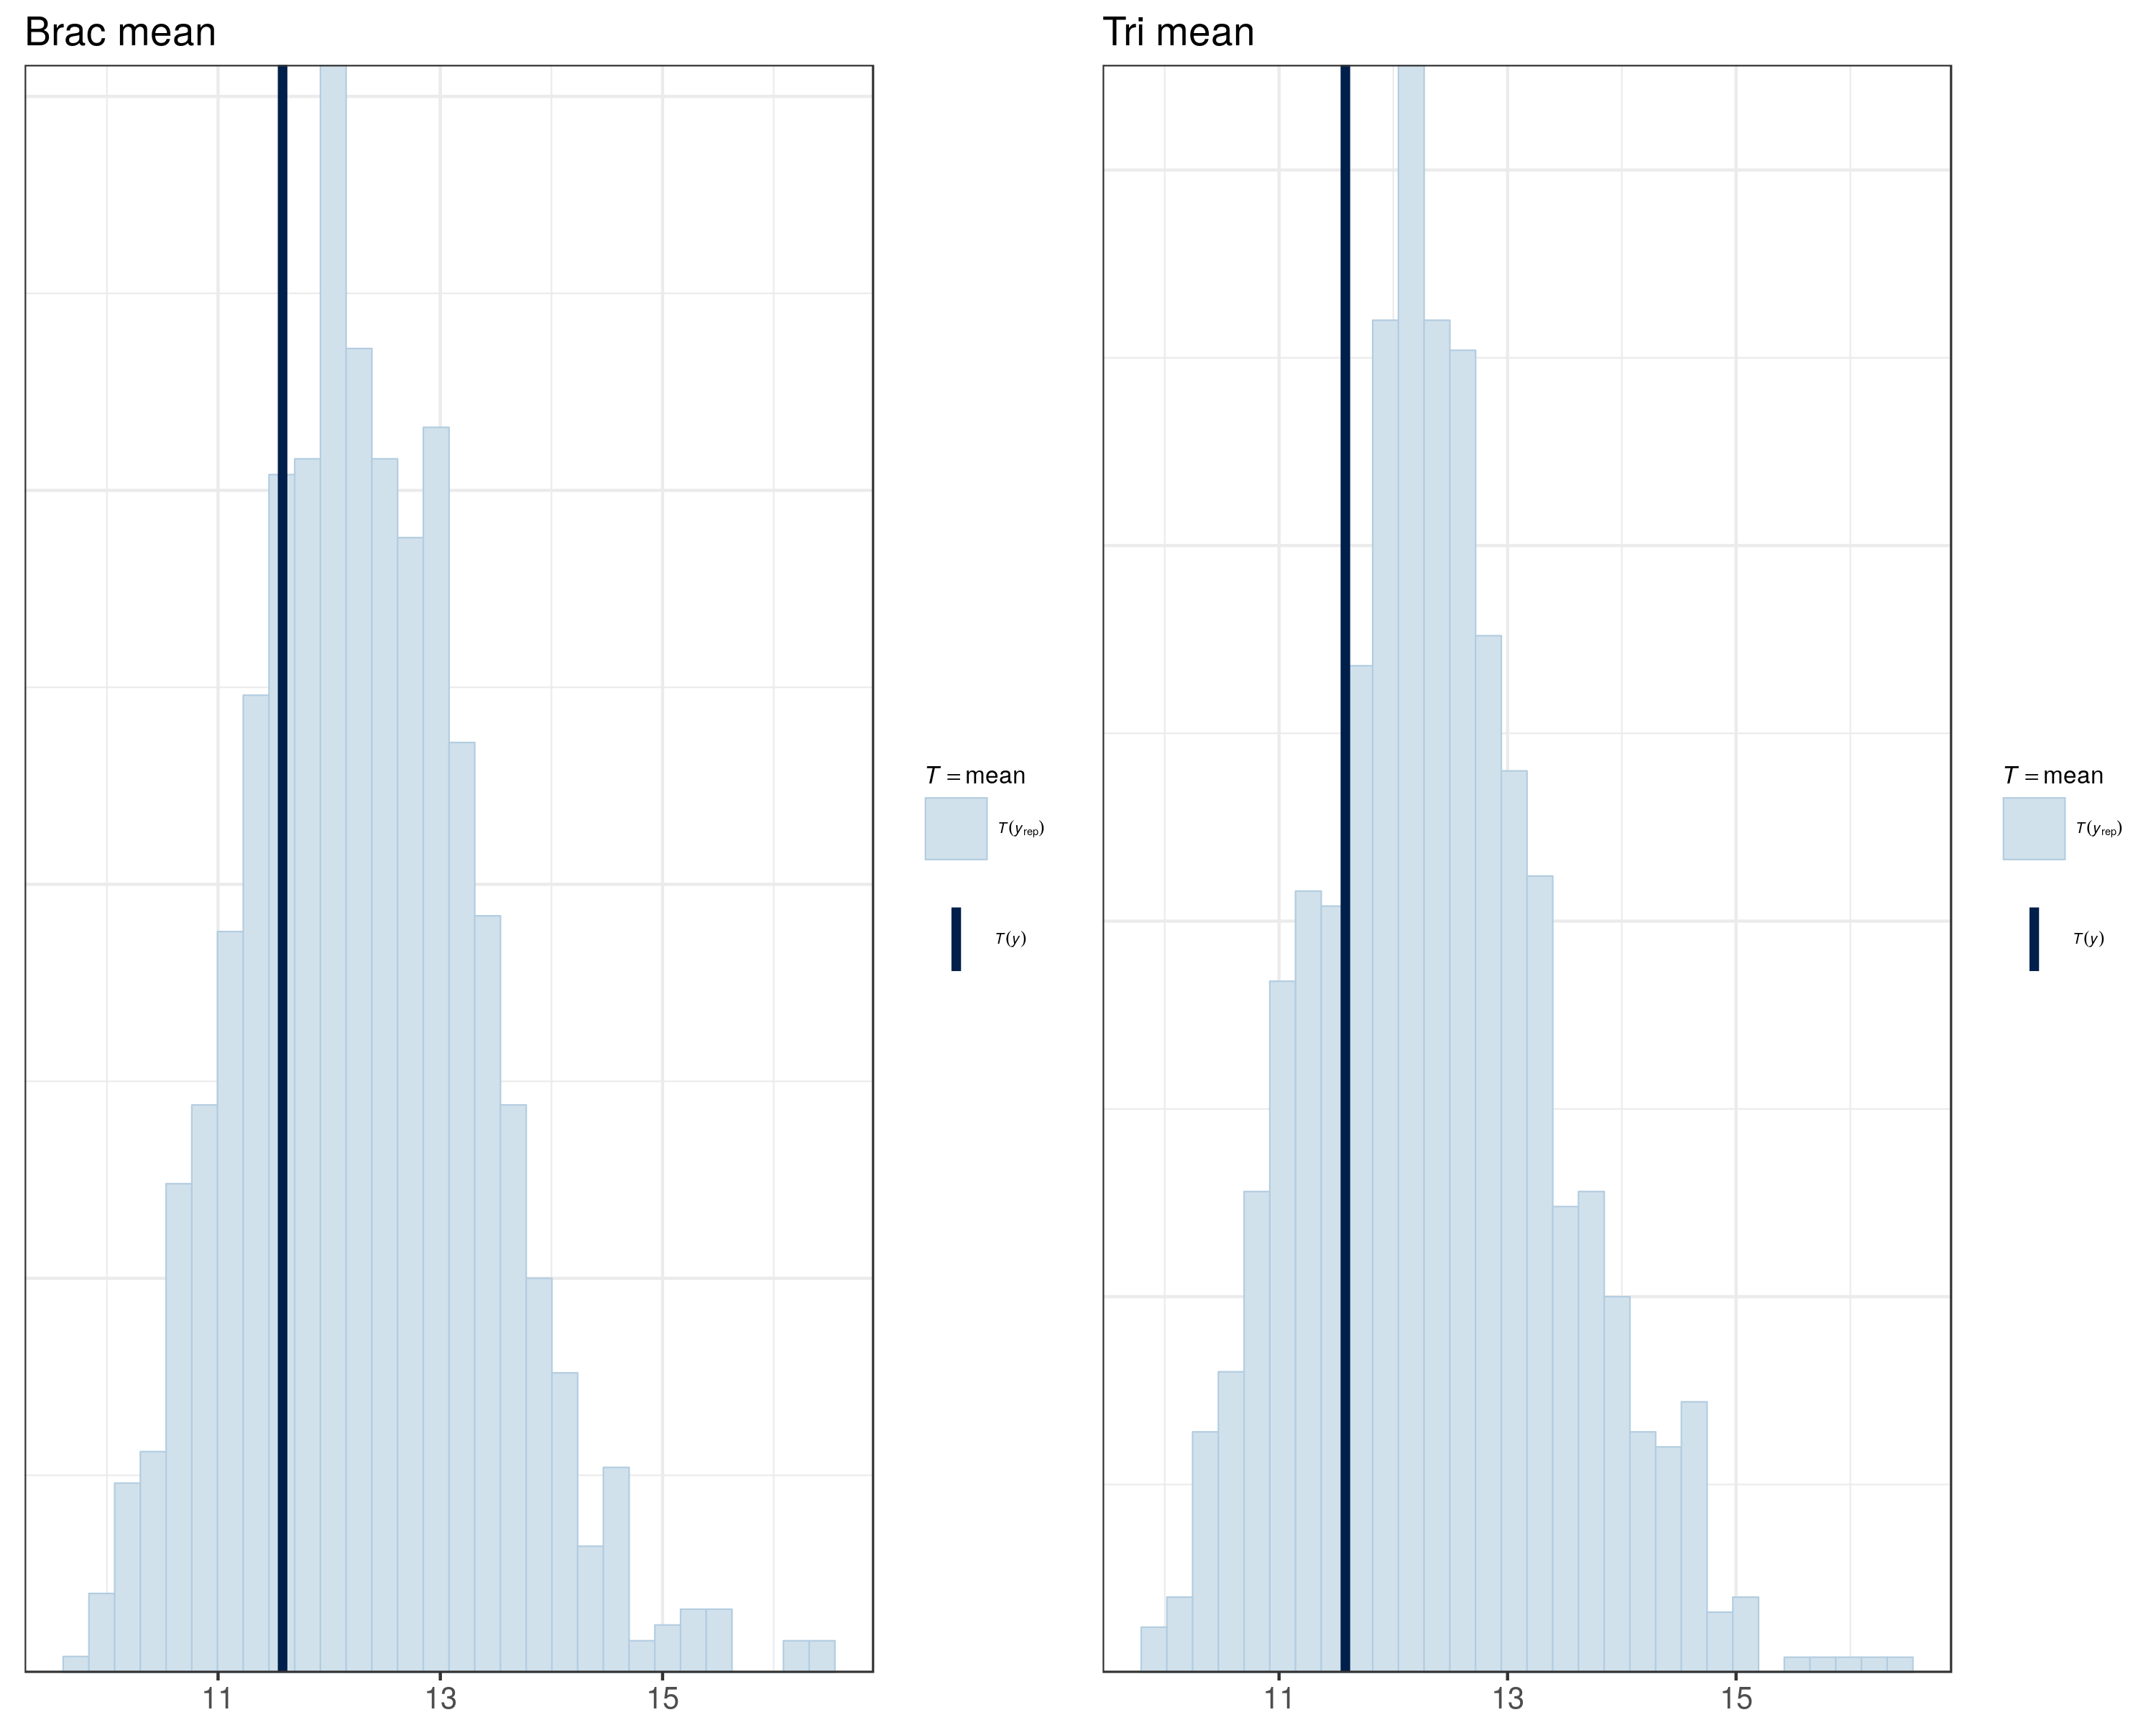
\includegraphics[width=\textwidth,height=0.5\textheight,keepaspectratio=true]{figure/ppc_mean_diversity}
  \caption{Posterior predictive results comparing the observed mean diversity of a geological unit for each of the studied taxonomic groups to a distribution of 1000 estimates from datasets simulated from the posterior predictive distribution of our models. Model adequacy is determined by how similar the posterior predictive distribution is to the observed value. In all cases, our models appear able to reproduce to observed means.}
  \label{fig:ppc_mean}
\end{figure}

Comparison of the observed standard deviation estimates for each of the taxonomic datasets to the posterior predictive distributions of our model fits show that our model is slightly over estimating the scale of our data, though not to a necessarily concerning degree (Fig. \ref{fig:ppc_sd}). Count data can frequently be over dispersed and have a standard deviation to mean ratio greater than 1; this reality is the reason we chose to use a truncated Negative-Binomial as opposed to a Poisson distribution because the addition of a second parameter allows us to model this overdispersion CITATIONS. While our model is not too different from the data, there is room for improvement in modeling the actual dispersion of geologic unit diversity.
% sd
\begin{figure}[ht]
  \centering
  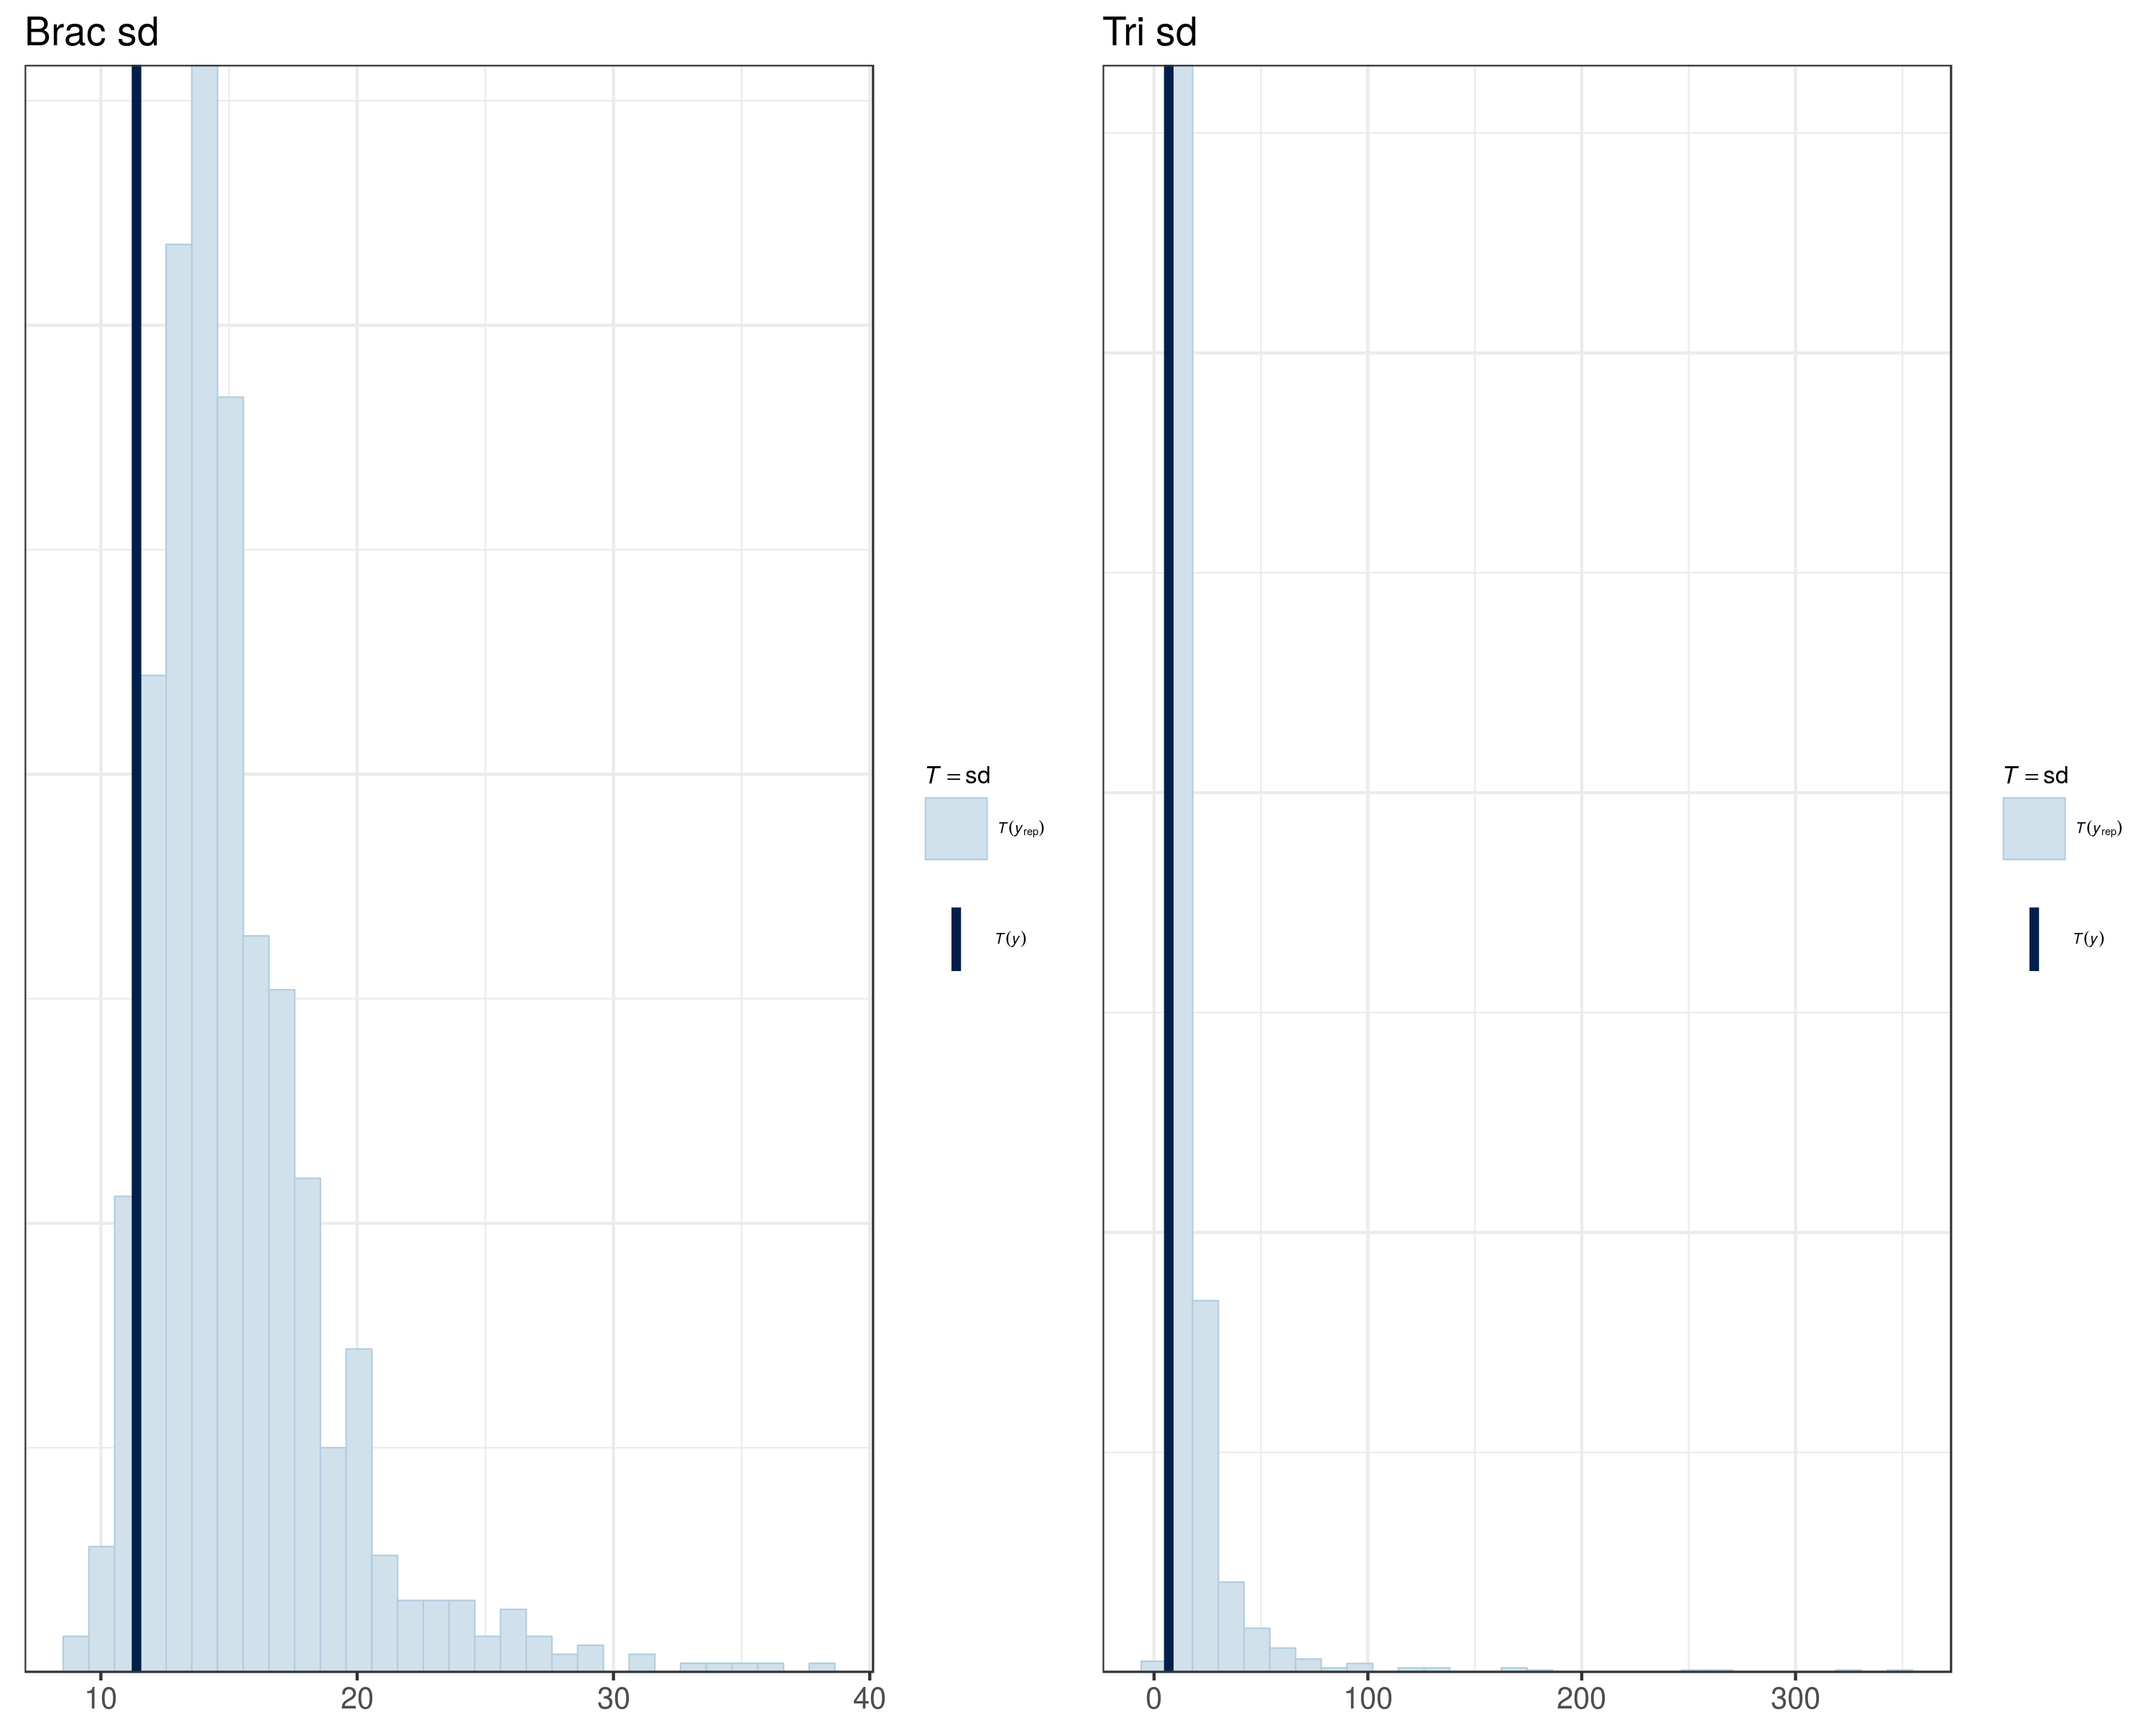
\includegraphics[width=\textwidth,height=0.5\textheight,keepaspectratio=true]{figure/ppc_sd_diversity}
  \caption{Posterior predictive results comparing the observed standard deviation diversity of a geological unit for each of the studied taxonomic groups to a distribution of 1000 estimates from datasets simulated from the posterior predictive distribution of our models. Model adequacy is determined by how similar the posterior predictive distribution is to the observed value. In all cases, our models appear able to reproduce to observed standard deviations.}
  \label{fig:ppc_sd}
\end{figure}


Comparisons of the empirical probability density functions for each of the taxonomic groups to the posterior predictive distribution of density functions generated by our model fits indicate that our model is very capable of recapitulating the observed data for nearly its entire range (Fig. \ref{fig:ppc_dens}). There are, however, minor but noticable differences between the posterior predictive distribution and the empirical data. For example, the posterior predictive distribution for Anthozoa slightly underestimates the number of units with diversity approximately 8. A similar underestimate is observable when comparing the posterior predictive distibution to the empirical data at unit diversity of approximately 11, and Brachiopoda at unit diversity of approximately 11. However, the posterior predictive distributions of our models fit the data well in nearly all cases, indicating that our model is potentially capturing some aspects of the data generating process.
\begin{figure}[ht]
  \centering
  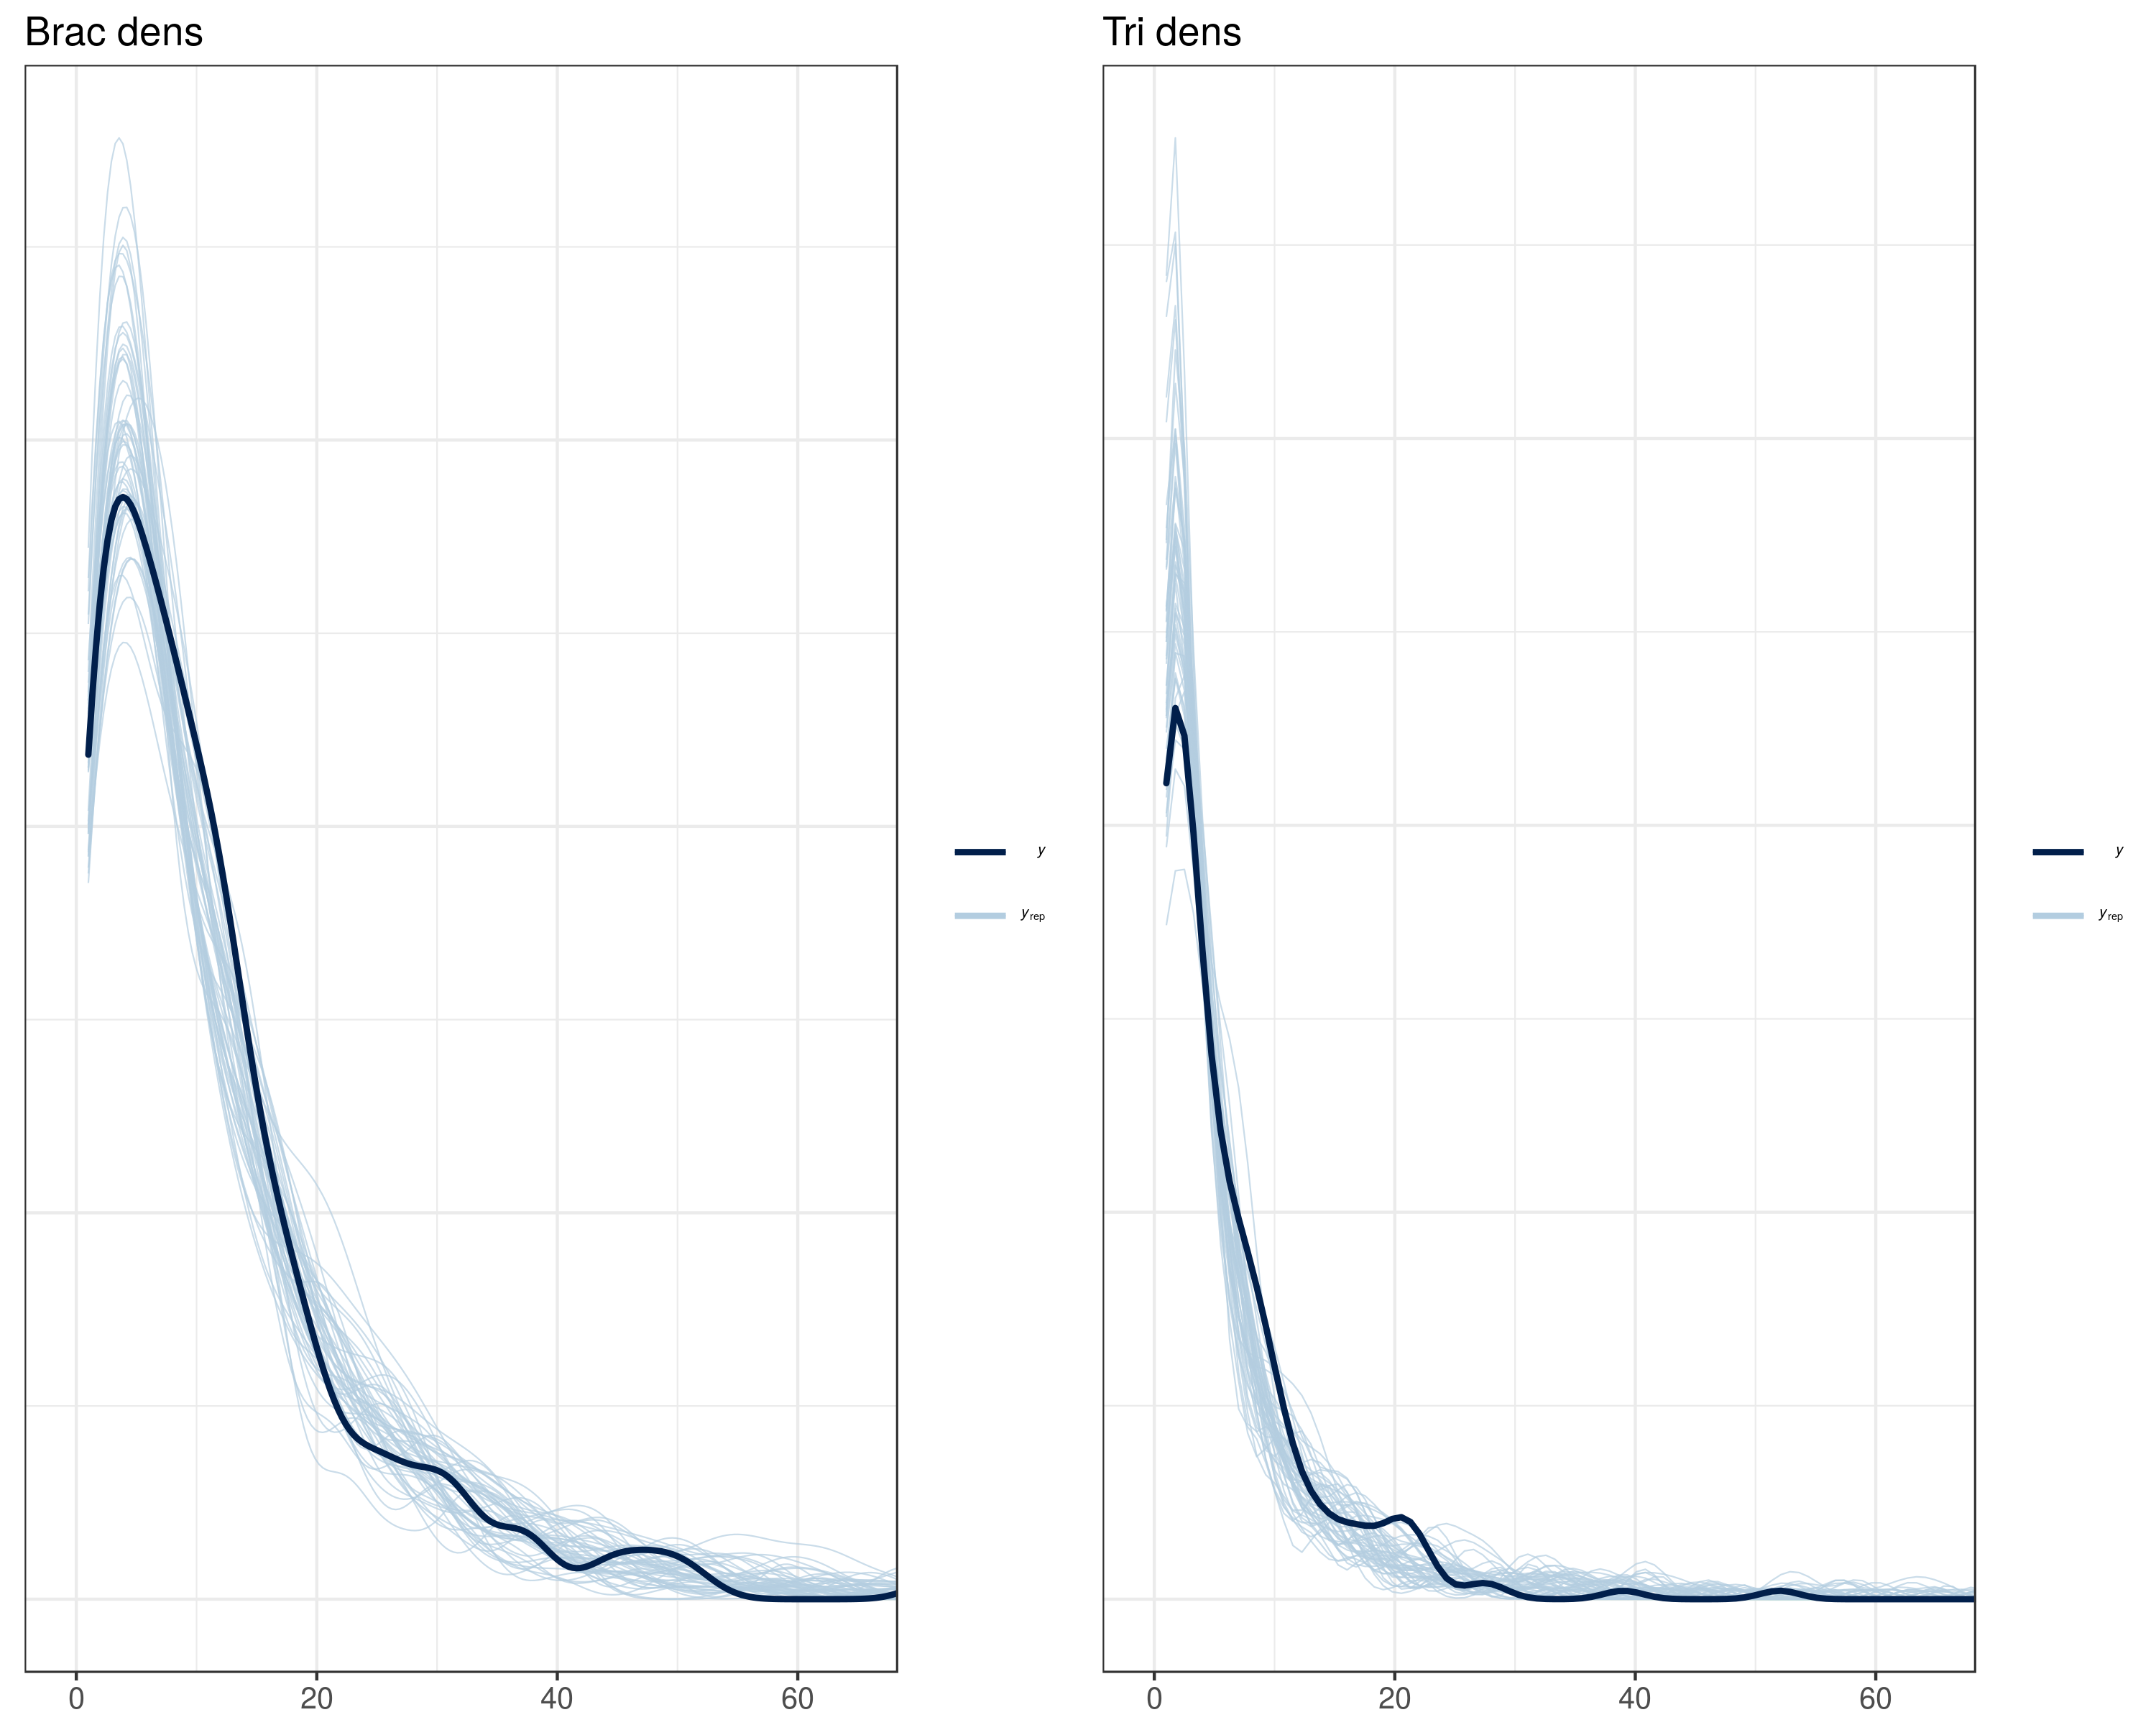
\includegraphics[width=\textwidth,height=0.5\textheight,keepaspectratio=true]{figure/ppc_dens_zoom_diversity}
  \caption{Posterior predictive results comparing the empirical probability density of a geological unit for each of the studied taxonomic groups to a distribution of 1000 probability densities from datasets simulated from the posterior predictive distribution of our models. Model adequacy is determined by how similar the posterior predictive distribution is to the observed value. In all cases, our models appear able to almost reproduce to observed ecdf-s.}
  \label{fig:ppc_dens}
\end{figure}


%The cummulative distribution function is description of the normalized rank order accumulation of the data. 
%\begin{figure}[ht]
%  \centering
%  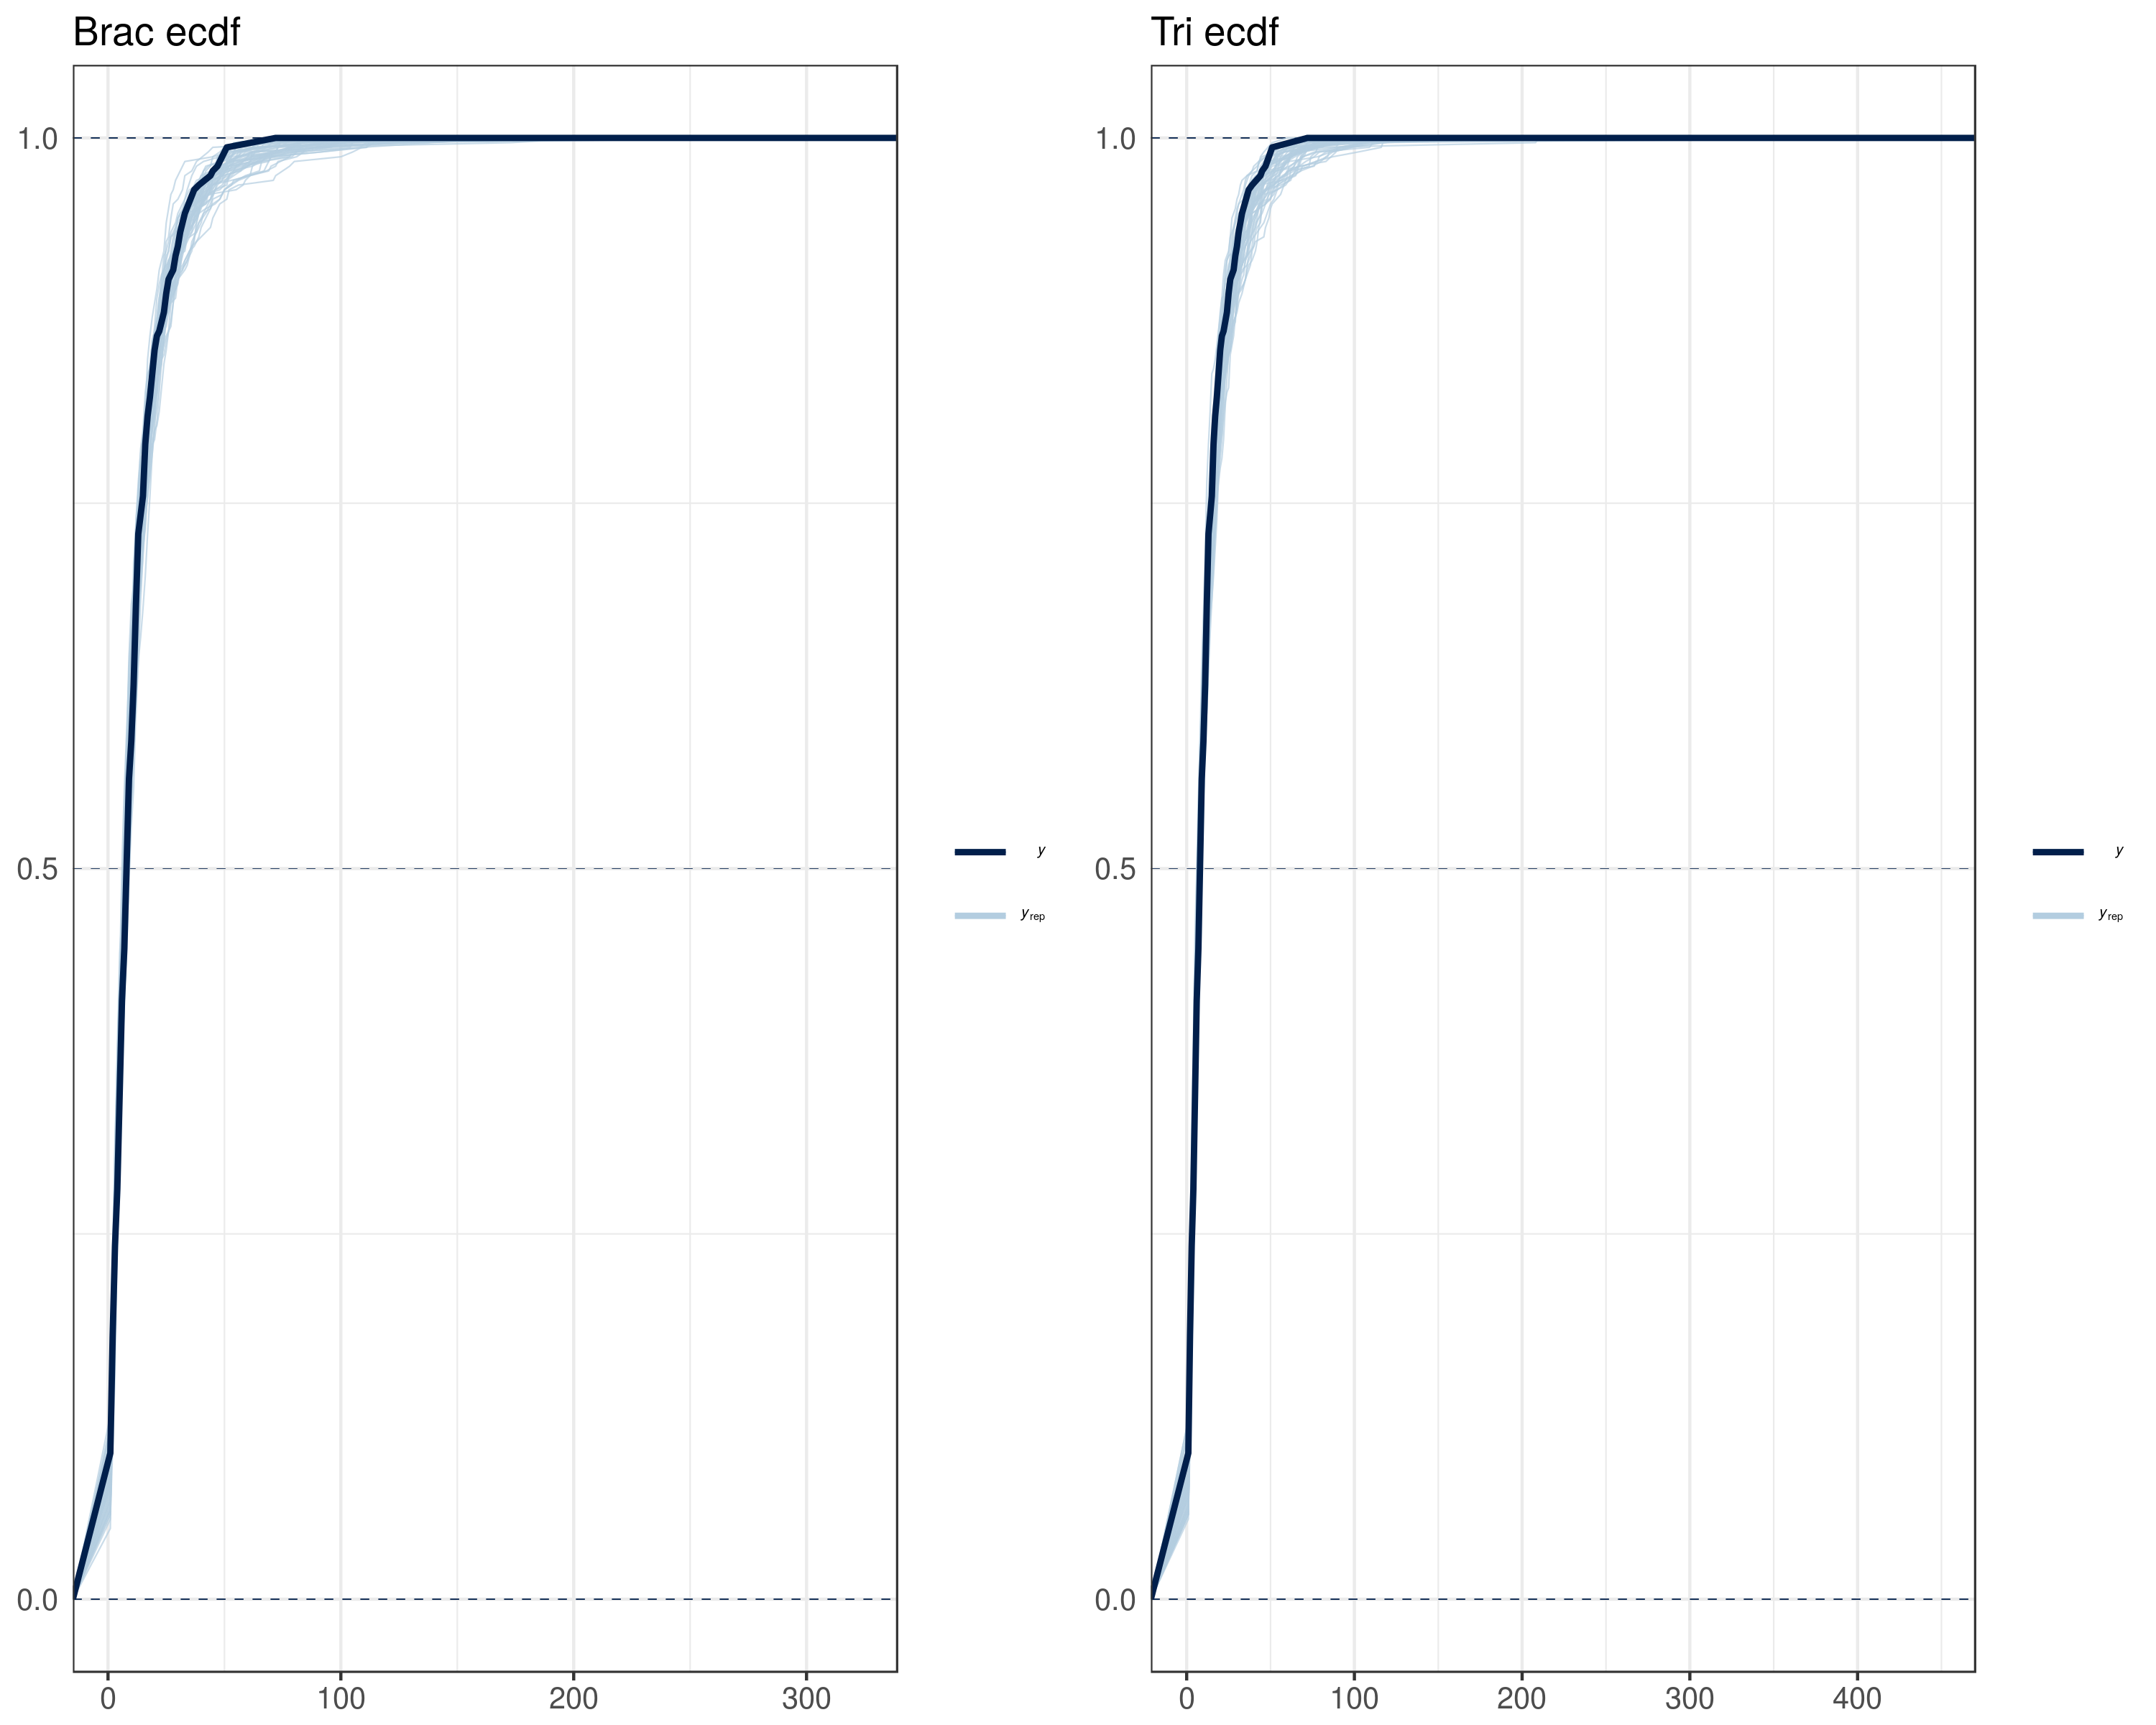
\includegraphics[width=\textwidth,height=0.5\textheight,keepaspectratio=true]{figure/ppc_ecdf_diversity}
%  \caption{Posterior predictive results comparing the empirical cummulative distribution function (ecdf) of a geological unit for each of the studied taxonomic groups to a distribution of 1000 estimates from datasets simulated from the posterior predictive distribution of our models. Model adequacy is determined by how similar the posterior predictive distribution is to the observed value. In all cases, our models appear able to almost reproduce to observed ecdf-s.}
%  \label{fig:ppc_ecdf}
%\end{figure}






\subsection{Estimated versus observed unit diversity}
% what is the point of this section?
%   graph unit diversity by time bin
%   compare to estimate from model
%   this is like the ppc for group mean, but inside-out
%   if model has poor estimates for time bin
%     that bin is not like what we would expect based on our model
%   if we have good estimates for all bins
%     then we need to look at covariates to see if there are any switch patterns


% time series graph
% what does this graph represent?
%   geological unit diversity counts at time bins
%   comparison to posterior predictive mean est with 80CI
Comparison between observed unit diversity over time and our models' estimates of mean unit diversity for those time steps reveals broad congruence (Fig. \ref{fig:time_div}). At no point does our model have a spurious or unrealistic estimate of mean geologic unit taxonomic diversity. This congruence gives us confidence in estimating the probability of the Hirnantian (1) having lower average unit diversity than the times directly before and after, and (2) having lower average unit diversity than the average unit diversity of the late Ordovician and the Silurian. 
\begin{figure}[ht]
  \centering
  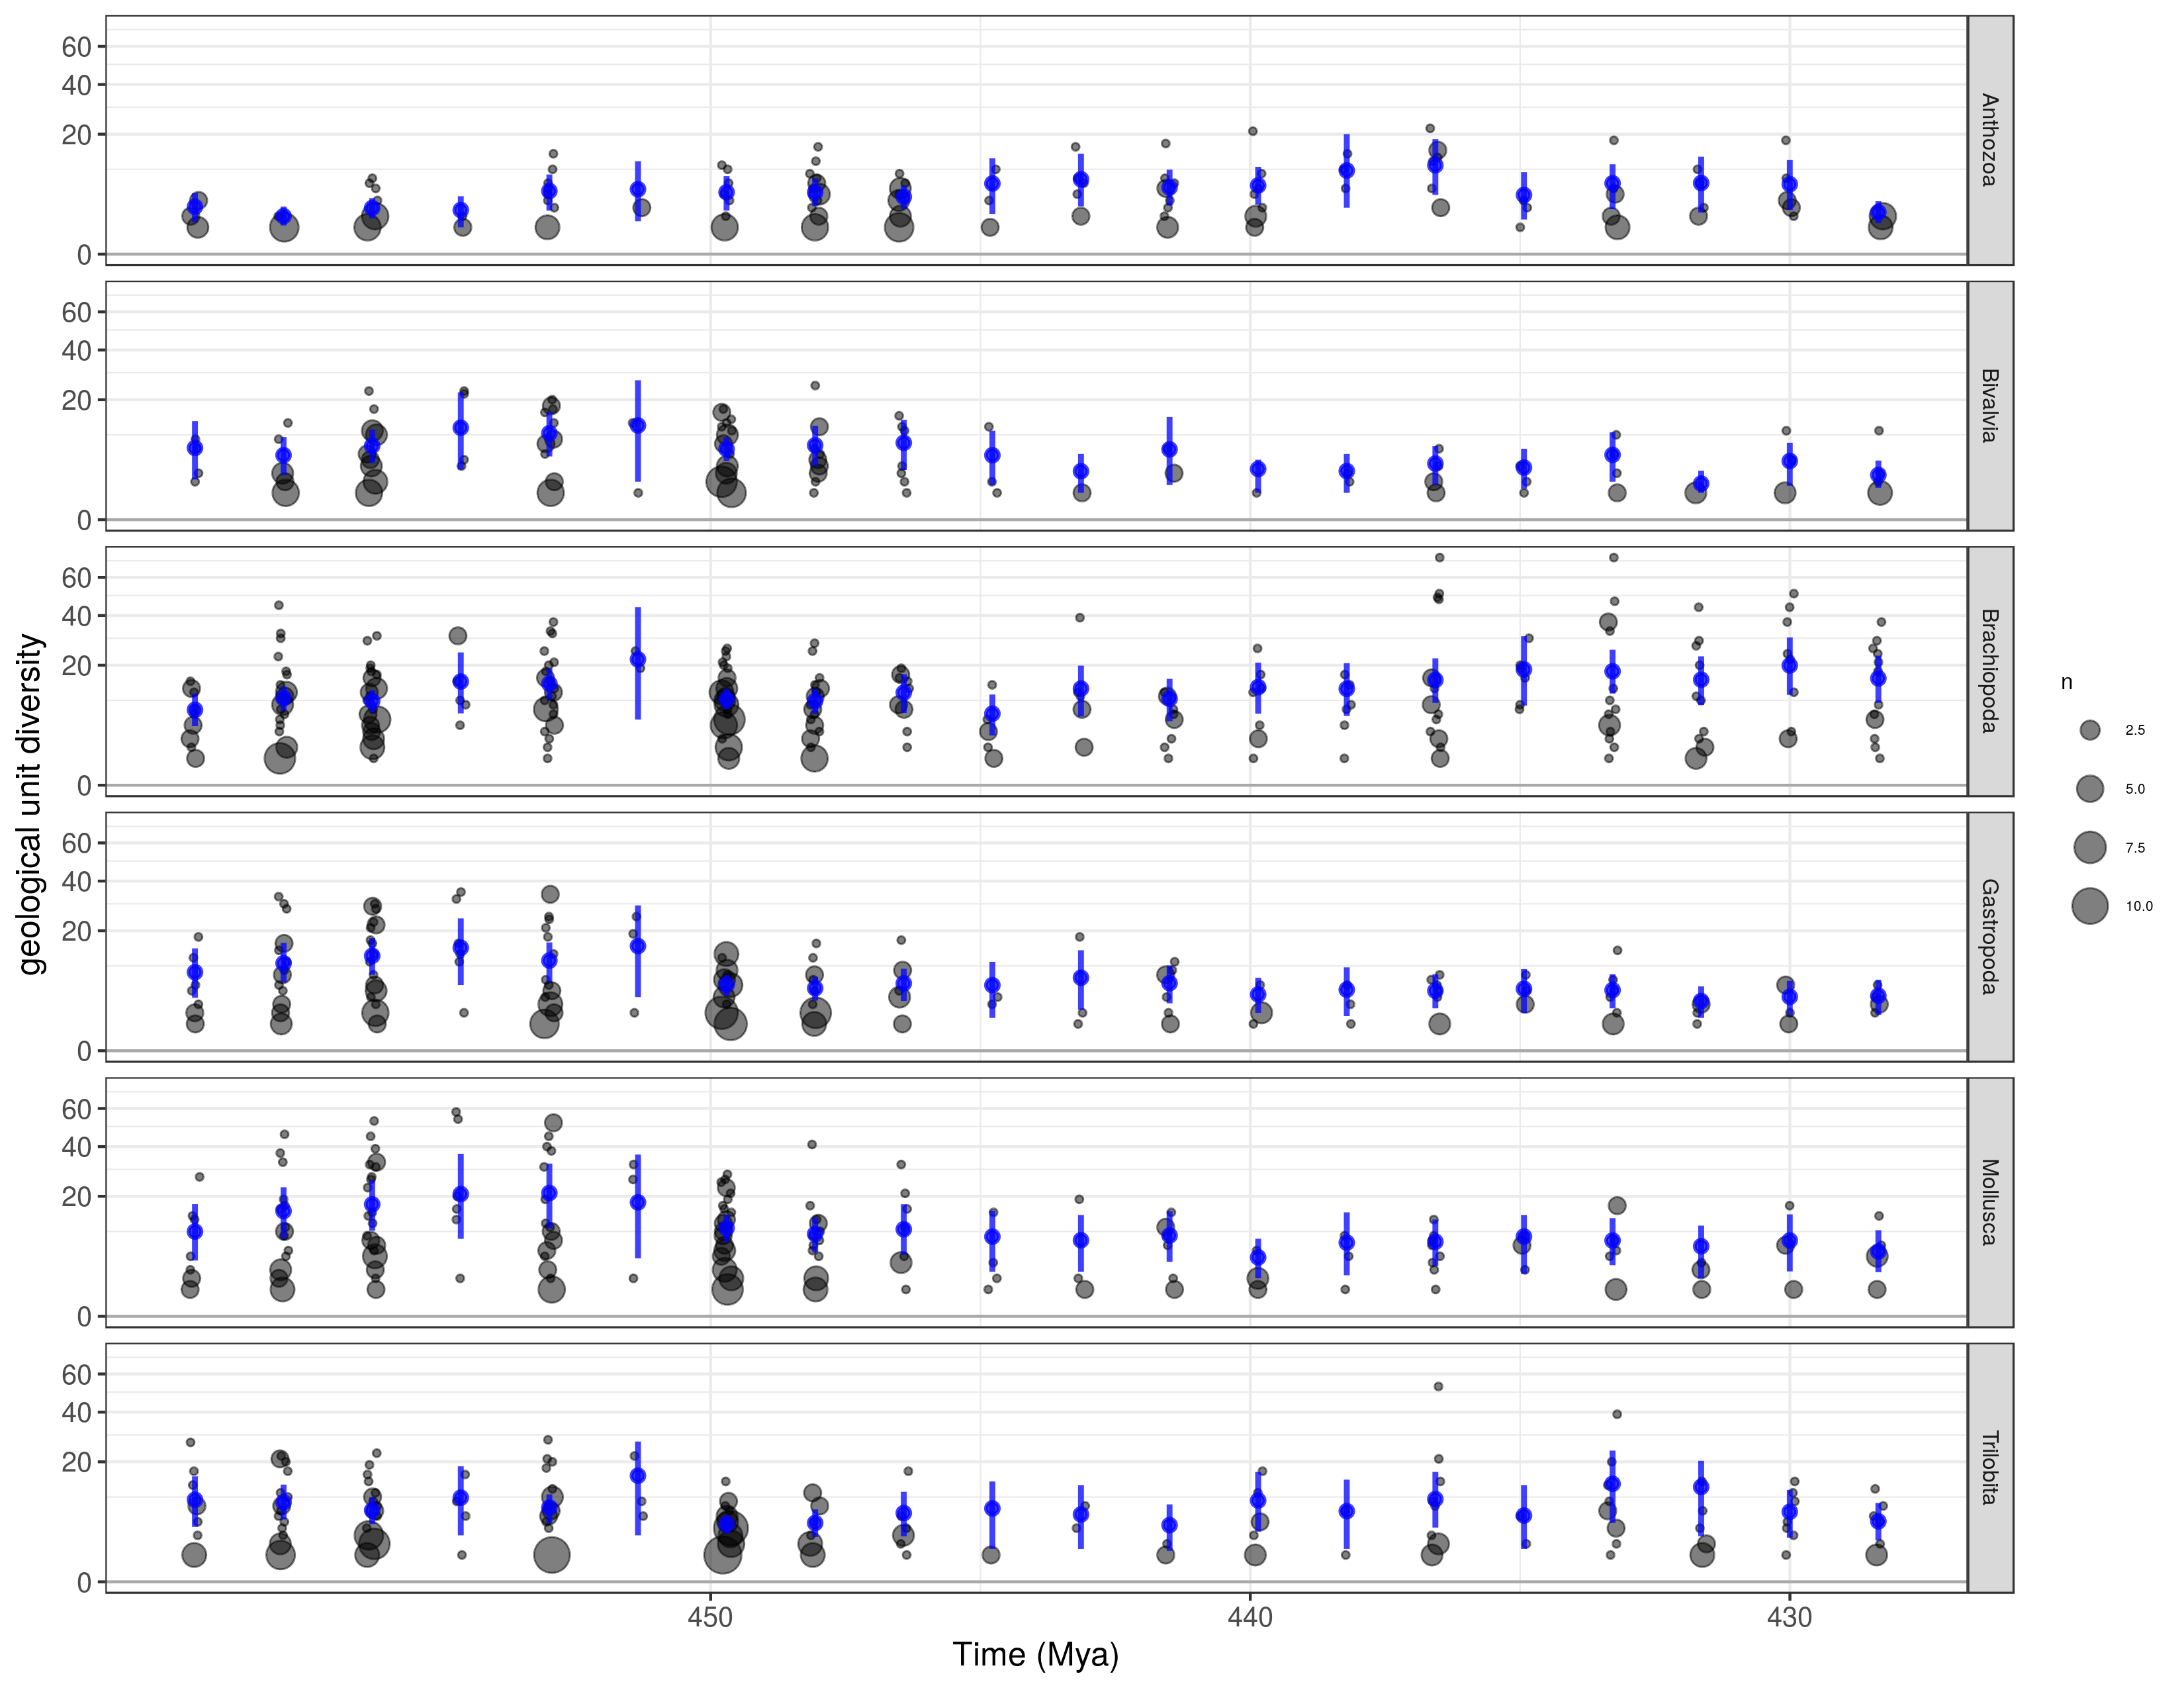
\includegraphics[width=\textwidth,height=0.5\textheight,keepaspectratio=true]{figure/unitdiv_time_diversity}
  \caption{Geological unit diversity though time and the expected diversity (with 80\% credible interval) as estimated from our models. Unit diversity is presented as partially transparent points and our jittered in the y-axis to improve readability. Point size is proportional to the number of units in that interval that have identical unit diversity. The dashed grey line corresponds to the onset of the Hirnantian geological stage, while the dashed-dotted grey line corresponds to the end of the Ordovician epoch and the start of the Silurian epoch.}
  \label{fig:time_div}
\end{figure}

We tested the probability that geologic units during the Hirnantian have lower expected unit diversity than the times immediately before and after by testing all advacent time bins (Fig. \ref{fig:diff_div}). For each adjacent time bins, we estimated the probability that the earlier time bin (time \(t\)) has a greater expected duration than the later time bin (time \(t + 1\)). Our analysis demonstrates that, for most comparisons, the expected unit diversity of Hirnantian time bin is not expected with high probability to be different from the time units immediately preceeding and following it. 


\begin{figure}[ht]
  \centering
  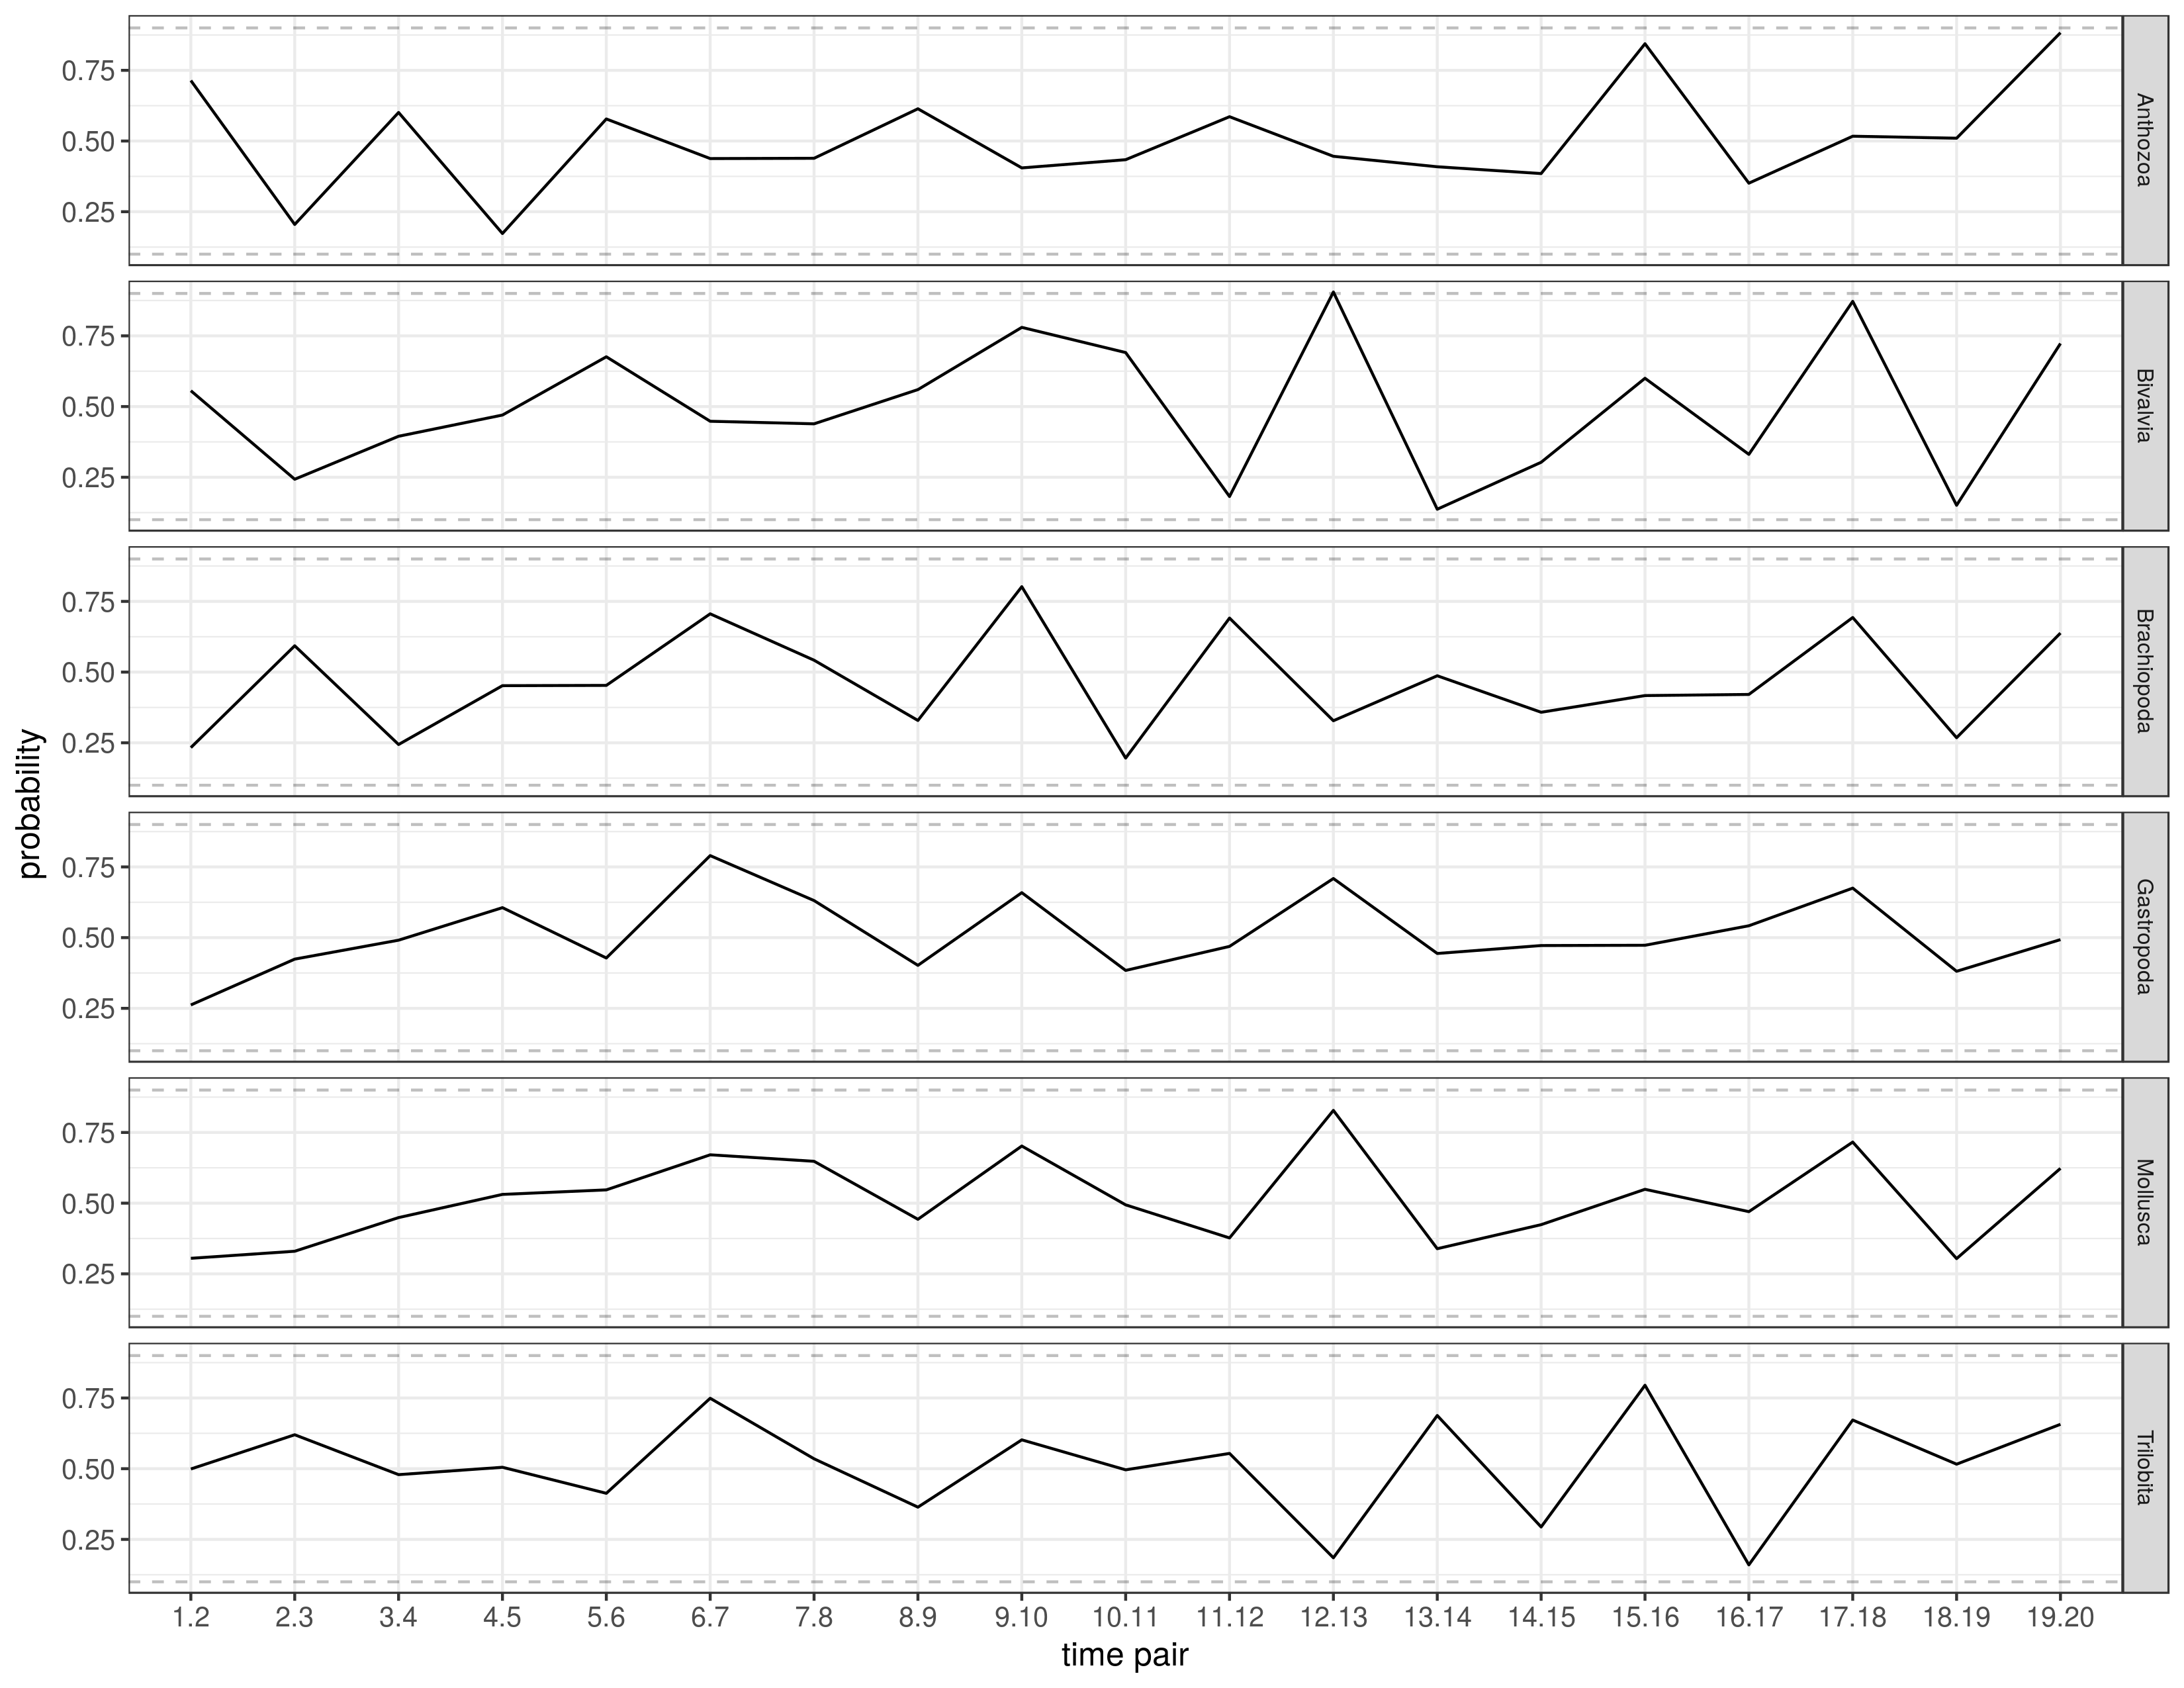
\includegraphics[width=\textwidth,height=0.5\textheight,keepaspectratio=true]{figure/unitdiv_diff_diversity}
  \caption{Probability that our estimate of mean unit diversity at time \(t\) is greater than the estimate at time \(t + 1\). The dashed grey horizontal lines correspond to probability of 0.9 and 0.1; these are the thresholds we chose as indicating if a pair-wise difference is potentially larger (or smaller) than no-difference (\(P = 0.5\)), and worthy of further inspection.}
  \label{fig:diff_div}
\end{figure}

% covariance of effect change?



\subsection{Effects of geological covariates on estimated diversity}
% what is the point of this section?
%   we've estimated the effect of multiple covariates
%   these estimates are allowed to vary through time
%     temporal structure is taken into account
%   what is the general relationship? what happens during hirnantian?
%     if all units have the same relationship
%       and all good bin estimates
%         there is no change in unit diversity though time
%         there is no change in geol properties that affect unit diversity
%       and some bad bin estimates
%         our model can not explain these bins; something is going on here
%     if some units have diff relationships (sign change, effect loss)
%       and all good bin estimates
%         we capture the changing relationship between preservational context and observed diversity
%       and some bad bin estimates
%         our model can not explain these bins; something is going on here


% time series graph
% what does this graph represent?
%   effect of covariate on expected count over time
%   violin shows full posterior estimate
%   pointrange shows mean with 80CI
As stated earlier, for all taxonomic groups the intercept term is an estimate of the expected (log) diversity of geologic unit diversity with mean thickness, area, latitude, and a purely non-dolomitic carbonate lithology. The effects of thickness, area, and latitude correspond to the expected change in (log) geologic unit diversity per change of the covariate value in units of standard deviations. The effects of dolomite, fine and coarse siliciclastic correspond to the change associated with unit change to the logratio representing the lithological composition of interest \citep{Hron2012}.

Estimates of covariates effects over time demonstrate a gradual shift in effects over time and not a sudden shift during the Hirnantian or between the Ordovician and the Silurian (Fig. \ref{fig:time_cov}). Interestingly, the covariate that may demonstrate the biggest pattern associated with the Hirnantian is the effect of geologic unit areal extent which appears to decrease in effect for Bivalvia, Gastropoda, and Mollusca. 
\begin{figure}[ht]
  \centering
  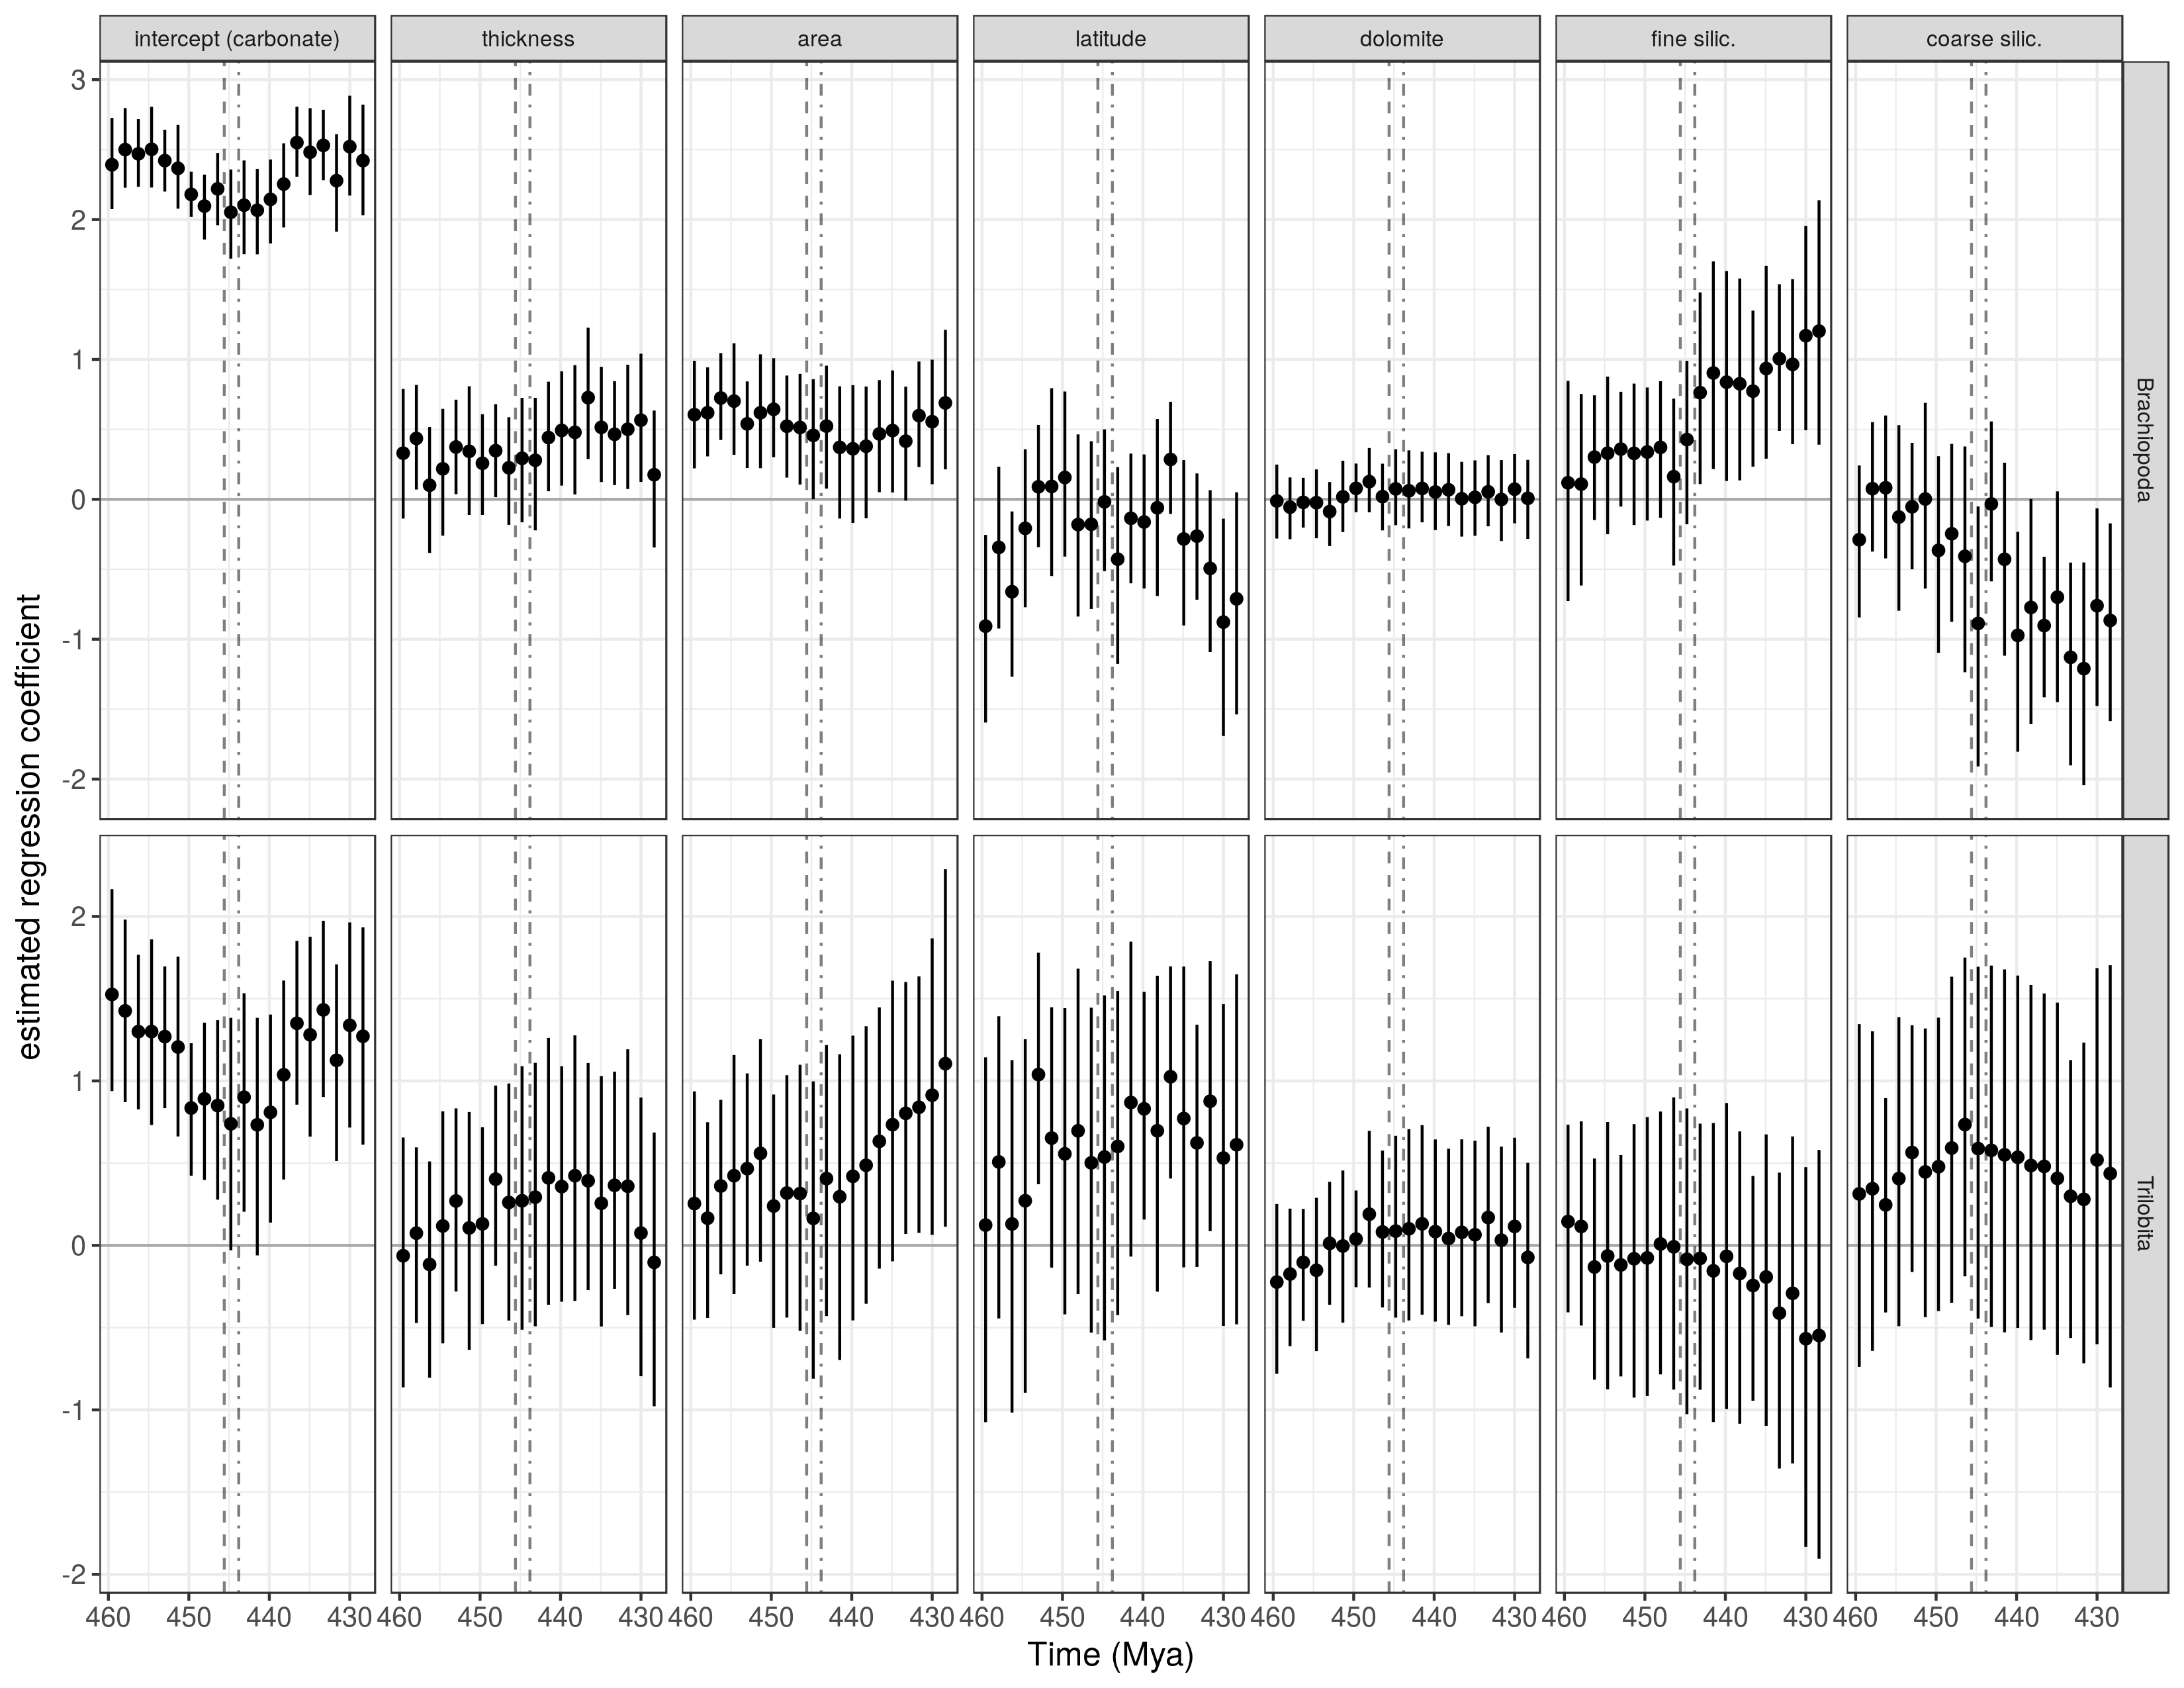
\includegraphics[width=\textwidth,height=0.5\textheight,keepaspectratio=true]{figure/cov_time_diversity}
  \caption{Estimates of all estimated covariate effect time series for each of the analyzed taxonomic groups, including intercept estimates. Points represent mean estimate along with a 80\% credible interval. The black horizontal line corresponds to no effect. Points are plotted at the mid-point of the discrete time interval.}
  \label{fig:time_cov}
\end{figure}


Similar to our earlier comparison of expected geologic unit diversity, we tested if any of the covariate effects estimated for one time bin (time \(t\)) were greater than the estimates from the following time bin (time \(t + 1\)). We find no strong evidence that the Hirnantian time bin is significantly different from the time bins immediately before and after (Fig. \ref{fig:diff_cov}). %There is only one example of a time unit comparison where we might expect a significant difference and that is for the estimated effect of areal extent on (log) geologic unit diversity between the 7th and 8th time bins. This is further evidence of gradual changes to the relationship between the properties of a geologic unit and its expected taxonomic diversity.
There are very few examples of one time bin having significantly different expected unit diversity than the one proceeding it. The intercept of our model fit to the Bivalvia dataset is expected to be greater during the second time unit than the third, though this difference is not associated with the Hirnantian time unit and thus is not very relevant to the thrust of our analysis. Similarly, we estimated a potentially significant difference the estimated effect of area in Mollusca, where the estimate for the seventh time unit is greater than the estimate for the eighth time unit.
\begin{figure}[ht]
  \centering
  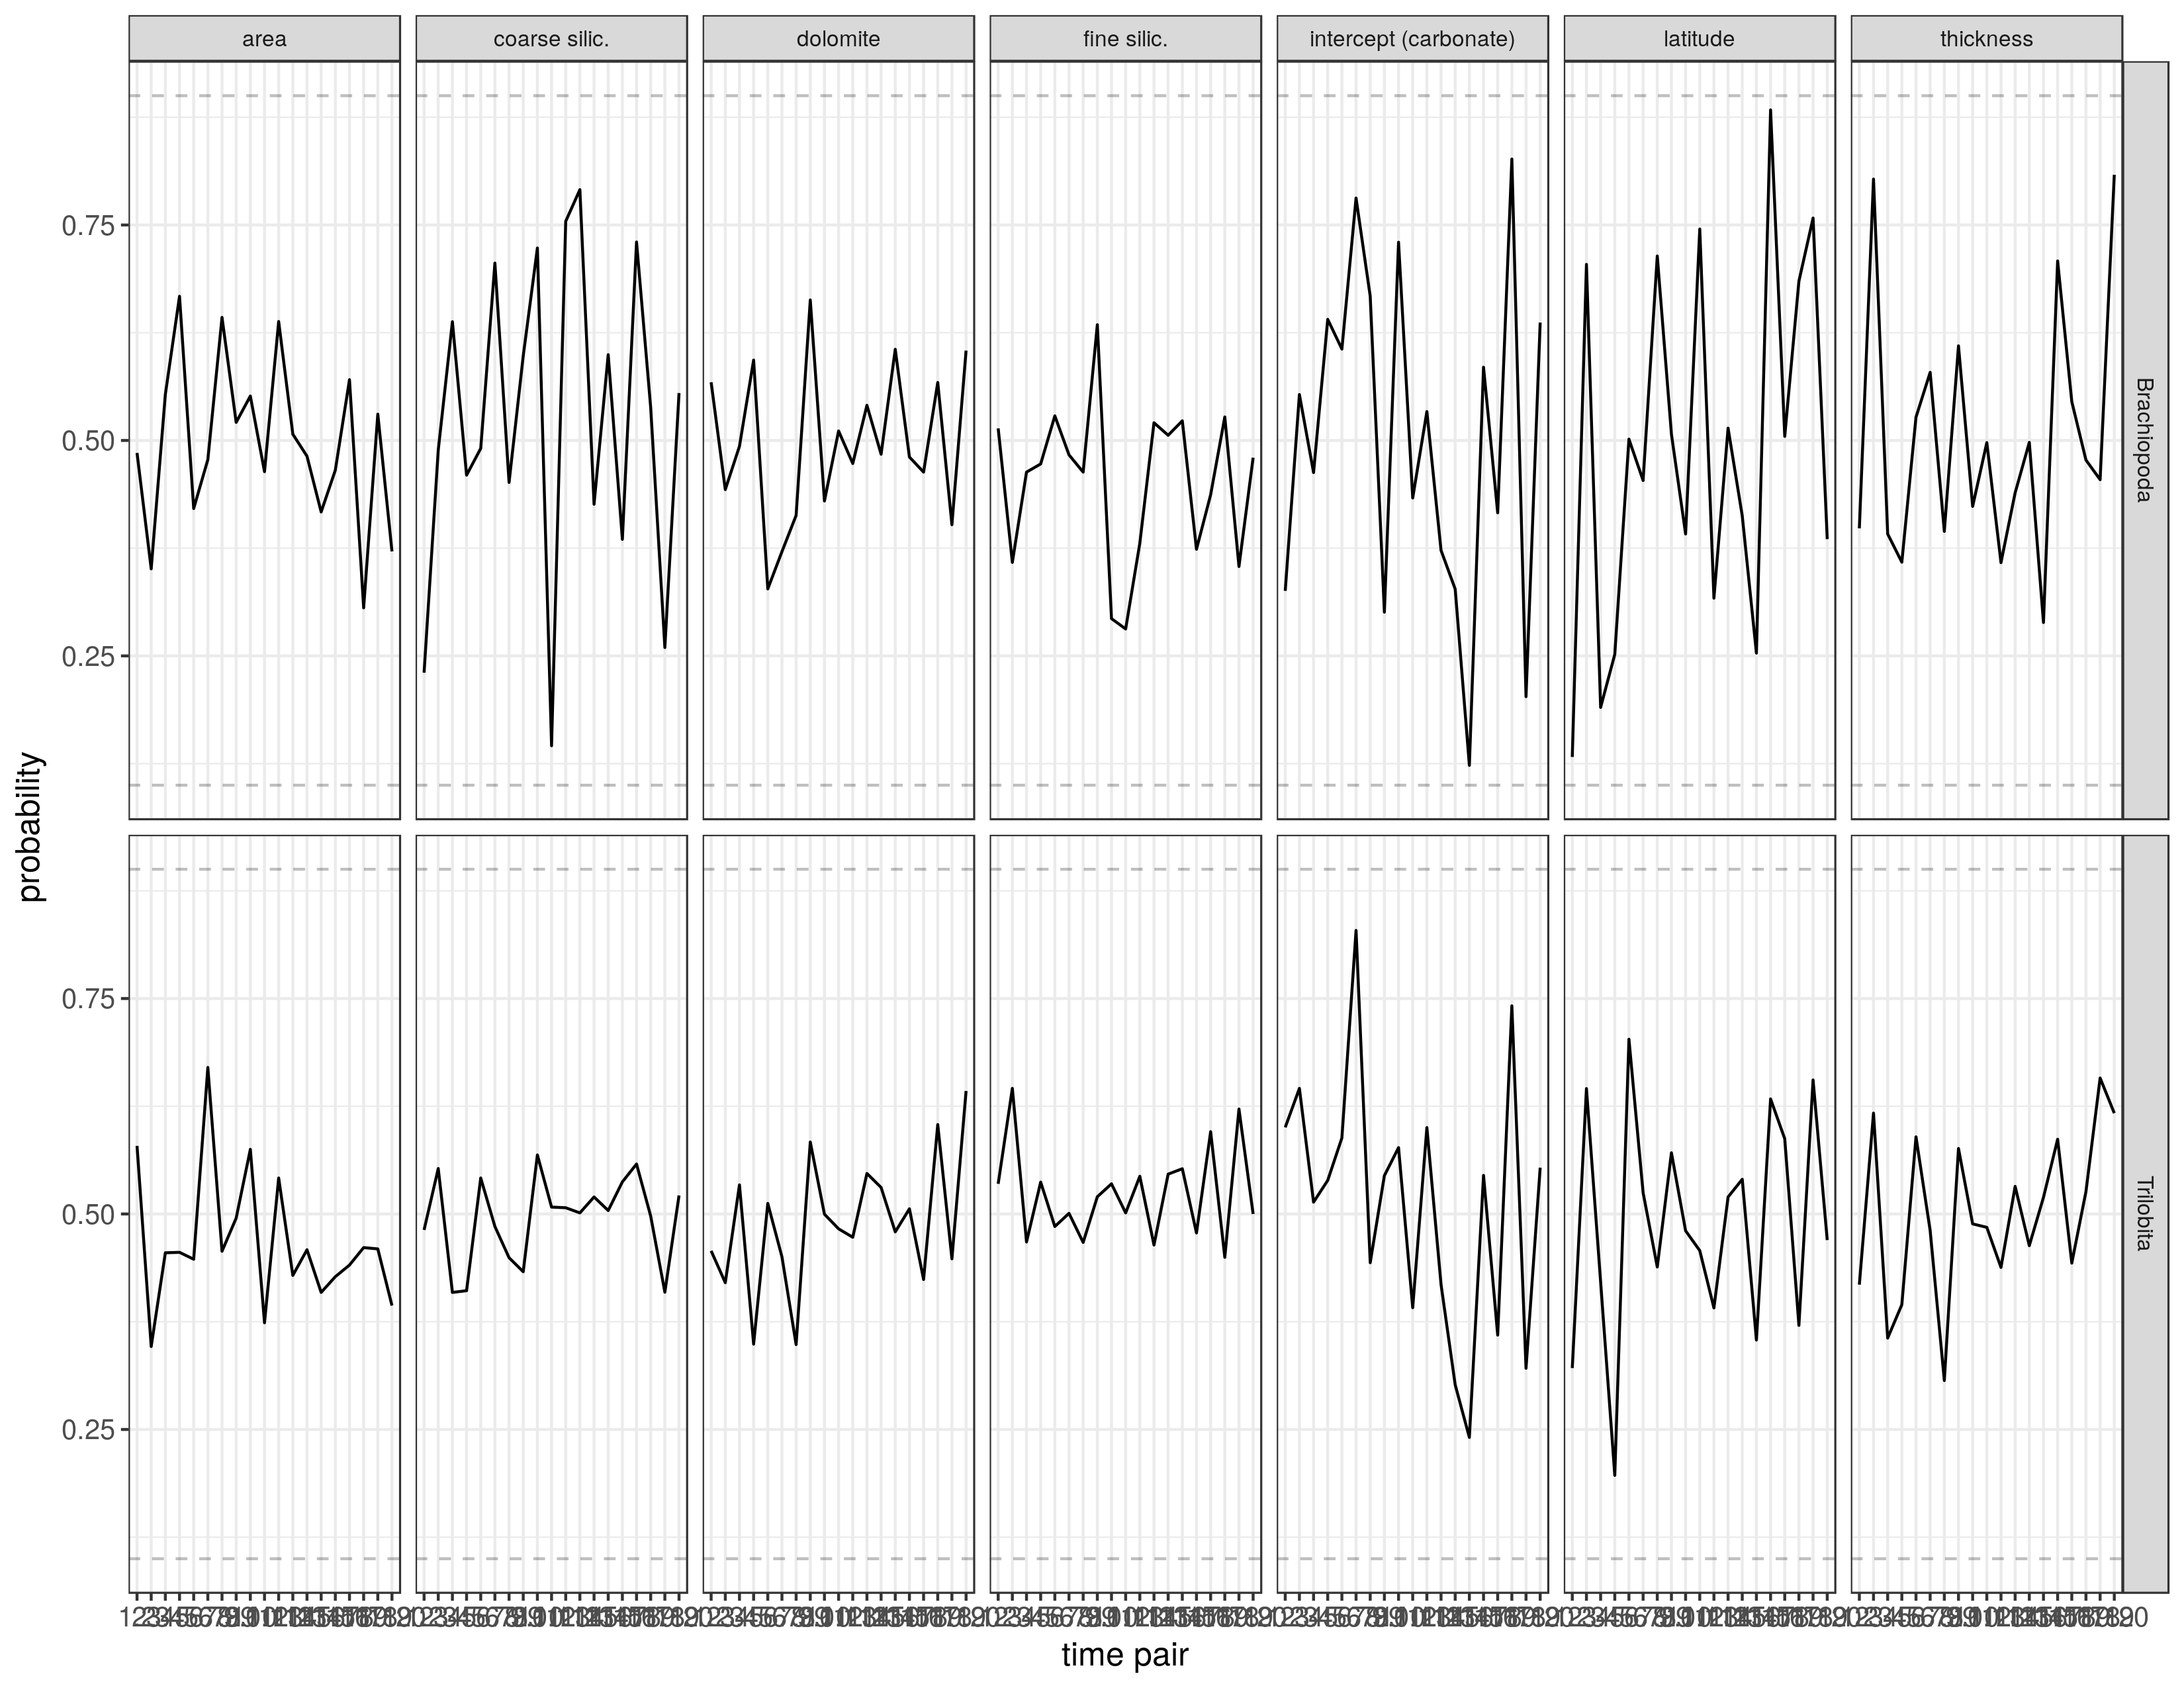
\includegraphics[width=\textwidth,height=0.5\textheight,keepaspectratio=true]{figure/cov_diff_diversity}
  \caption{Probability that a parameter estimate at time \(t\) is greater than the estimate at time \(t + 1\). The dashed grey horizontal lines correspond to probability of 0.9 and 0.1; these are the thresholds we chose as indicating if a pair-wise difference is potentially larger (or smaller) than no-difference (\(P = 0.5\)), and worthy of further inspection.}
  \label{fig:diff_cov}
\end{figure}


Of particular interest is if the Hirnantian has a lower expected unit diversity than the average of the Ordovician or Silurian. Additionally, we are interested in if the covariate estimates for the Hirnantian are different than those estimated for the rest of the Ordovician or Silurian. Here we calculate the probability that the expected unit diversity of the Hirnantian is less than the averages for the Ordovician or Silurian and compare those estimates to the probabilities that the covariate effects are less than the averages for the Ordovician or Silurian (Fig. \ref{fig:pvalue}). We find that in most cases there is no strong evidence (probability \(> 0.9\)) for the Hirnantian being significantly different from the averages of either the Ordovician or the Silurian. However, there is weak evidence (probability \(> 0.75\)) for some differences between the Hirnantian and the Ordovician or Silurian.

All of the following results are supported with only weak evidence and are thus of interest for future study of lithological and diversity differences associated with the Hirnantian.

For Brachiopoda, Gastropoda, and Mollusca the average diversity of geologic units in the Orodovician is estimated with weak support to be greater than the expected unit diversity of the Hirnantian. We find weak support for a lower effect of dolomite composition on Anthozoan unit diversity during the Hirnantian than the average of the Ordovician. Similarly, we find weak support for a lower intercept term and the effect of coarse siliciclastics for Brachiopoda, Gastropoda, Mollusca, and Trilobita in the Hirnantian than the average of the Ordovician. The intercept is also the effect of being a purely non-dolomitic carbonate unit. We also find marginal support for the effect of area on unit diversity of Bivalvia, Gastropoda, and Mollusca being greater for the average of the Ordovician than those units from the Hirnantian.


We do find evidence that Brachiopods are expected to have greater unit diversity during the Silurian than during the Hirnantian. This result is one of the strongest support results from this study. Bivalvia and Mollusca intercept weak evidence expected to be greater in Hirnantian than average Silurian. This is also the effect of being a purely non-dolomitic carbonate unit. Bivalvia and Mollusca are estimated to have a lower effect of geologic unit area during the Hirnantian than the average of the Silurian. Finally, there is marginal evidence for the intercept estimate for Brachiopoda during the Hirnantian is expected to be lower than the average estimated intercept for the Silurian.
\begin{figure}[ht]
  \centering
  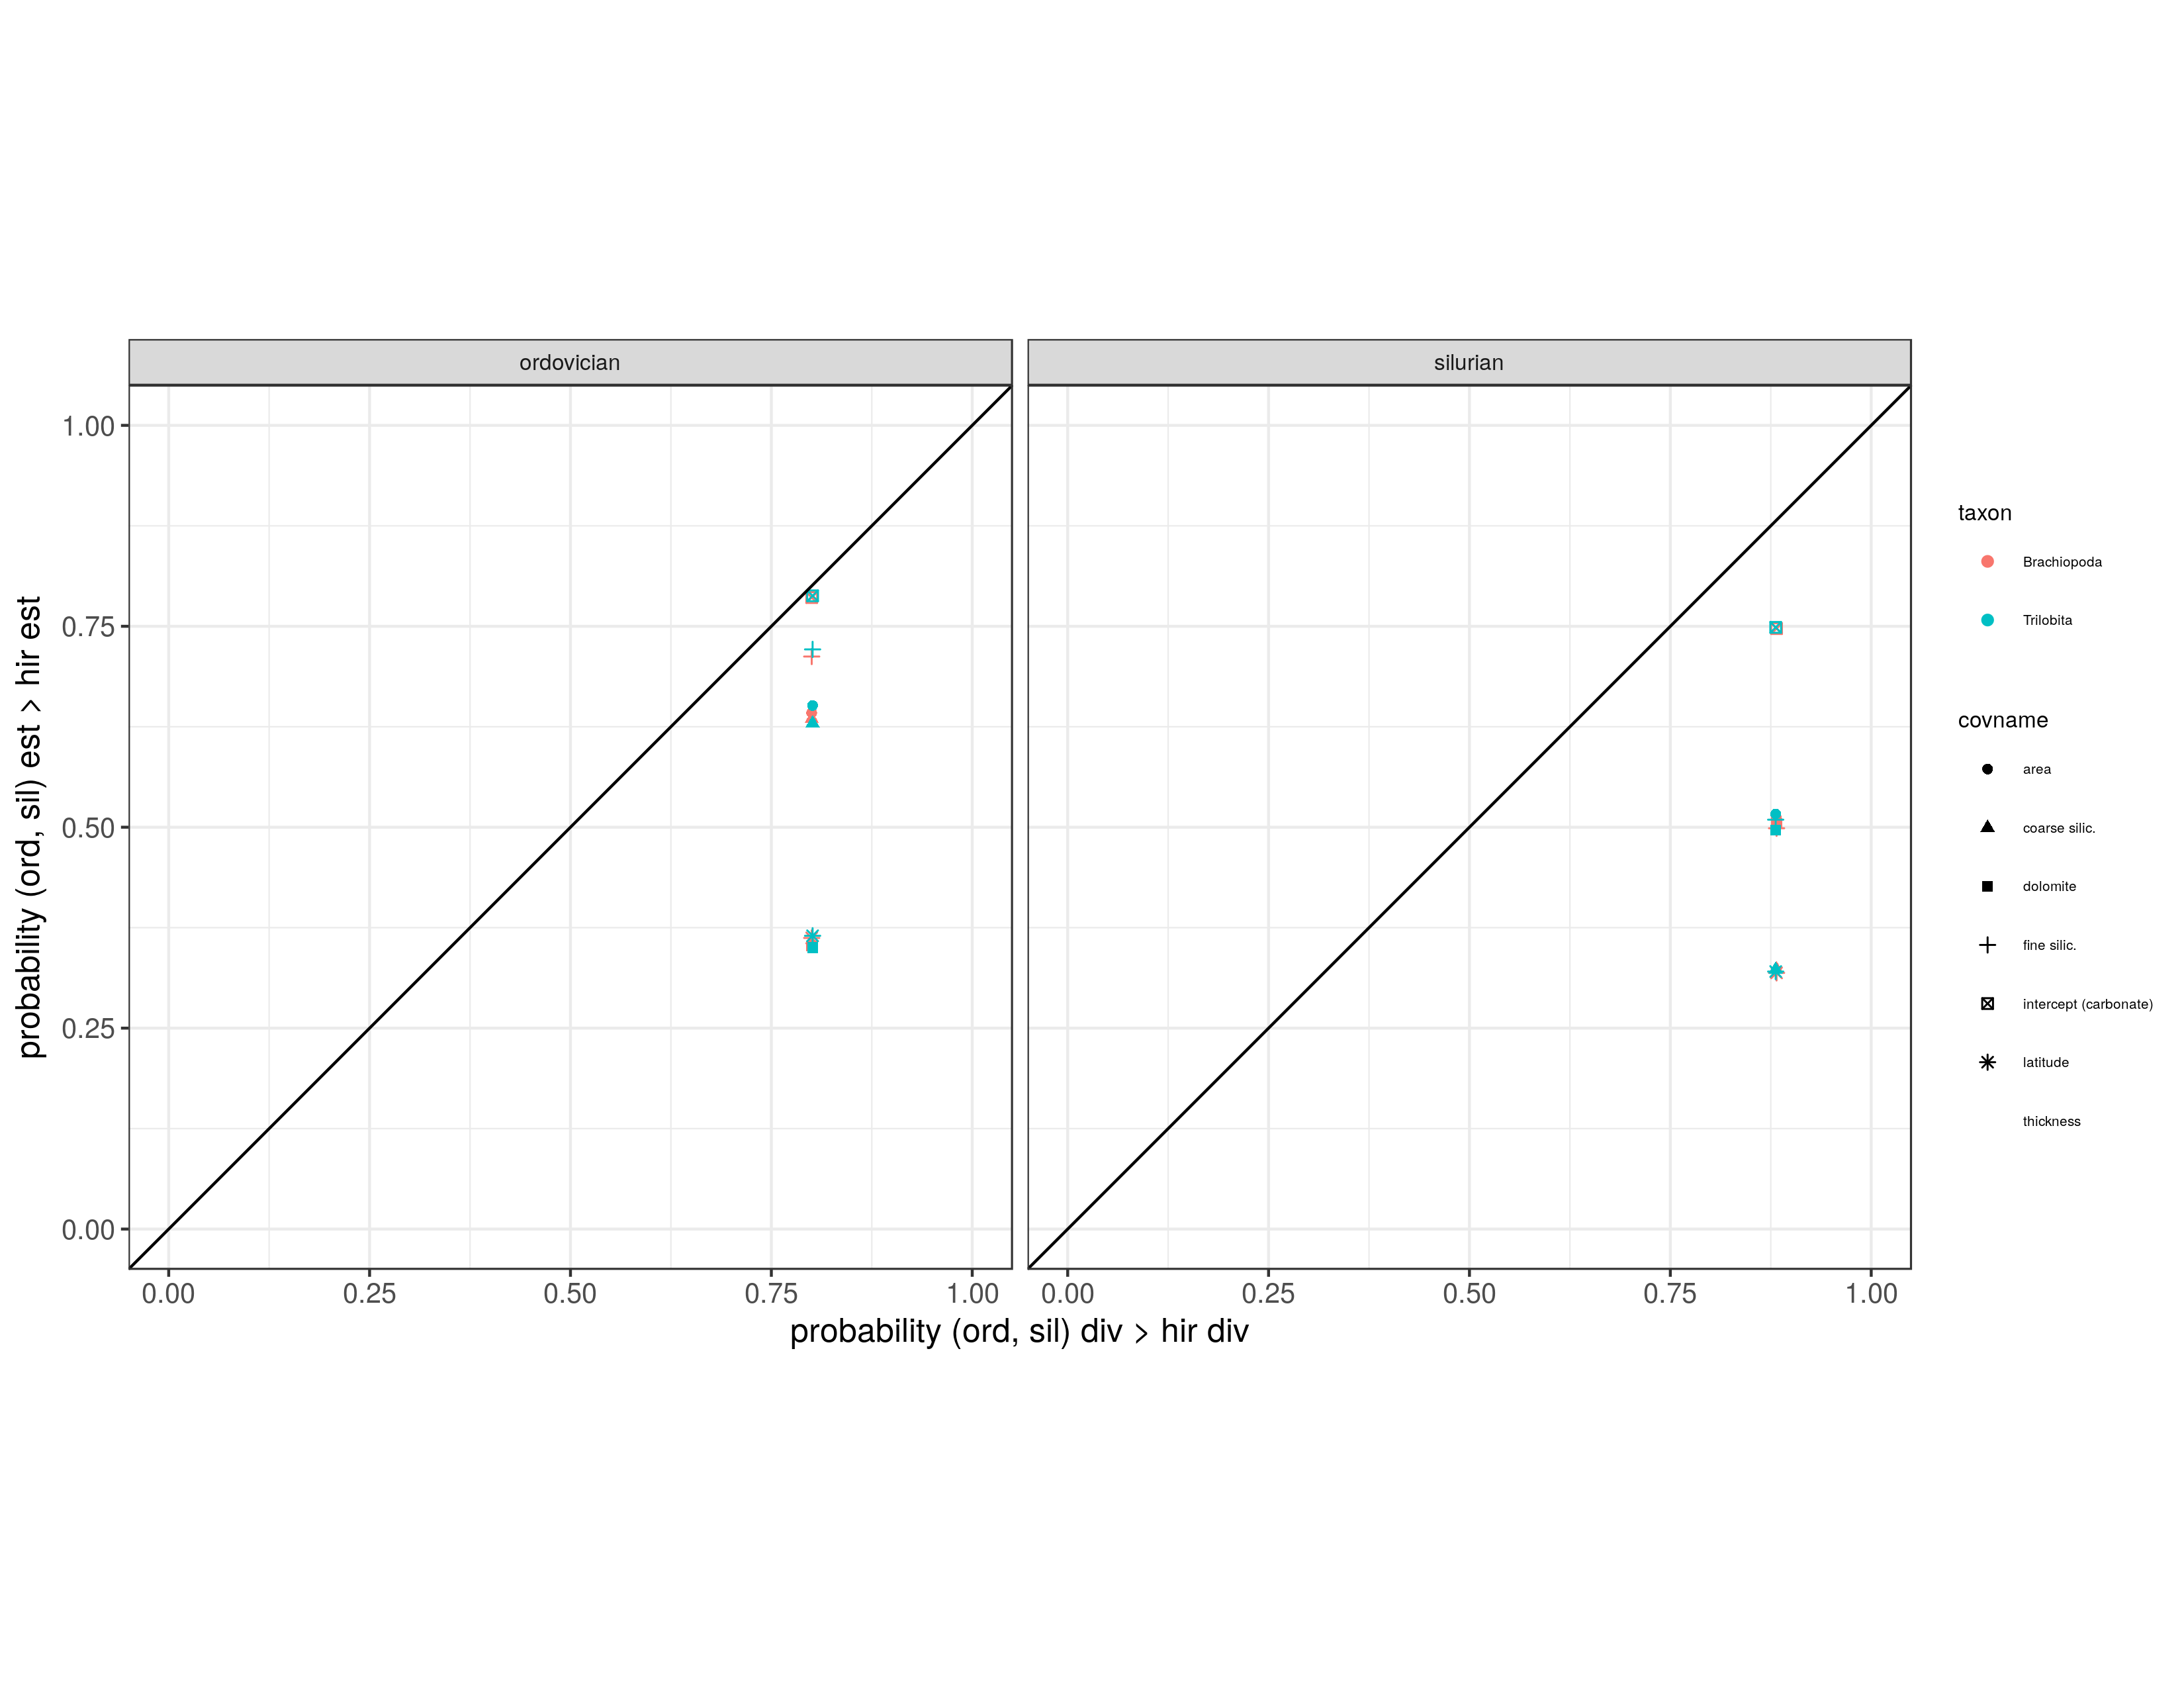
\includegraphics[width=\textwidth,height=0.5\textheight,keepaspectratio=true]{figure/compare_pval_diversity}
  \caption{Scatterplot of the estimated probability that geological unit diversity is lower during the Hirnantian than either the Ordovician (left facet) or the Silurian (right facet) vs the estimated probability that a covariate estimate is lower during the Hirnantian than either the Ordovician or the Silurian. For each of the taxonomic groups there is only one estimate for the probability of difference in diversity, but there are six probability estimates for each of the covariate effect parameters. }
  \label{fig:pvalue}
\end{figure}


\end{document}
